\definecolor{green}{cmyk}{0,0.25,0.5,0}
\definecolor{orange}{cmyk}{0,0.25,0.5,0}
\newcommand{\weblong}[2]{\href{#1}{#2}} % definition of long hyperreferences
\newcommand {\key}[1]{\textbf{\ttfamily{#1}}} % definition of key
\newcommand {\button}[1]{\textbf{\sffamily{#1}}} % definition of GUI button
\newcommand {\command}[1]{{\ttfamily{#1}}} % definition of console command
\newcommand {\excl}[1]{
	\begin{tabular}{r p{0.75\textwidth}}
	\hspace*{5mm}\LARGE{\textcolor{green}{$!$
	%\ArrowBoldDownRight
}} & #1\\		
\end{tabular}
}
\newcommand {\photo}[3]
{\begin{center}
  \includegraphics[width=0.5\textwidth]{img/#3}
\end{center}}		

\newcommand {\fg}{\FlightGear}

%%%%%%%%%%%%%%%%%%%%%%%%%%%%%%%%%%%%%%%%%%%%%%%%%%%%%%%%%%%%%%%%%%%%
\chapter{A Basic Flight Simulator Tutorial\label{basic}}
%%%%%%%%%%%%%%%%%%%%%%%%%%%%%%%%%%%%%%%%%%%%%%%%%%%%%%%%%%%%%%%%%%%%

\section{Foreword}
\label{sec:Foreword}
    
Aviation is about extremes:

\begin{itemize}
	\item An airplane is quite fragile and flies at high speeds. 
  Yet it is one of the safest forms of transport.
	\item Pilots must constantly follow rules and procedures. 
  Yet an airplane is a symbol of freedom.
	\item With a little training, flight a small aircraft is easy.
  Yet if a problem occurs, you must be able to resolve it in a  few seconds.
	\item Many flight tutorials are written with a lot of humor.
  Yet not taking flying seriously will bring you down to earth prematurely.
\end{itemize}
    
The aircraft used in this tutorial is the
\weblong{http://en.wikipedia.org/wiki/Cessna_172} {Cessna 172p}, the standard
aircraft in many real life flight schools and a great airplane:


\begin{center}
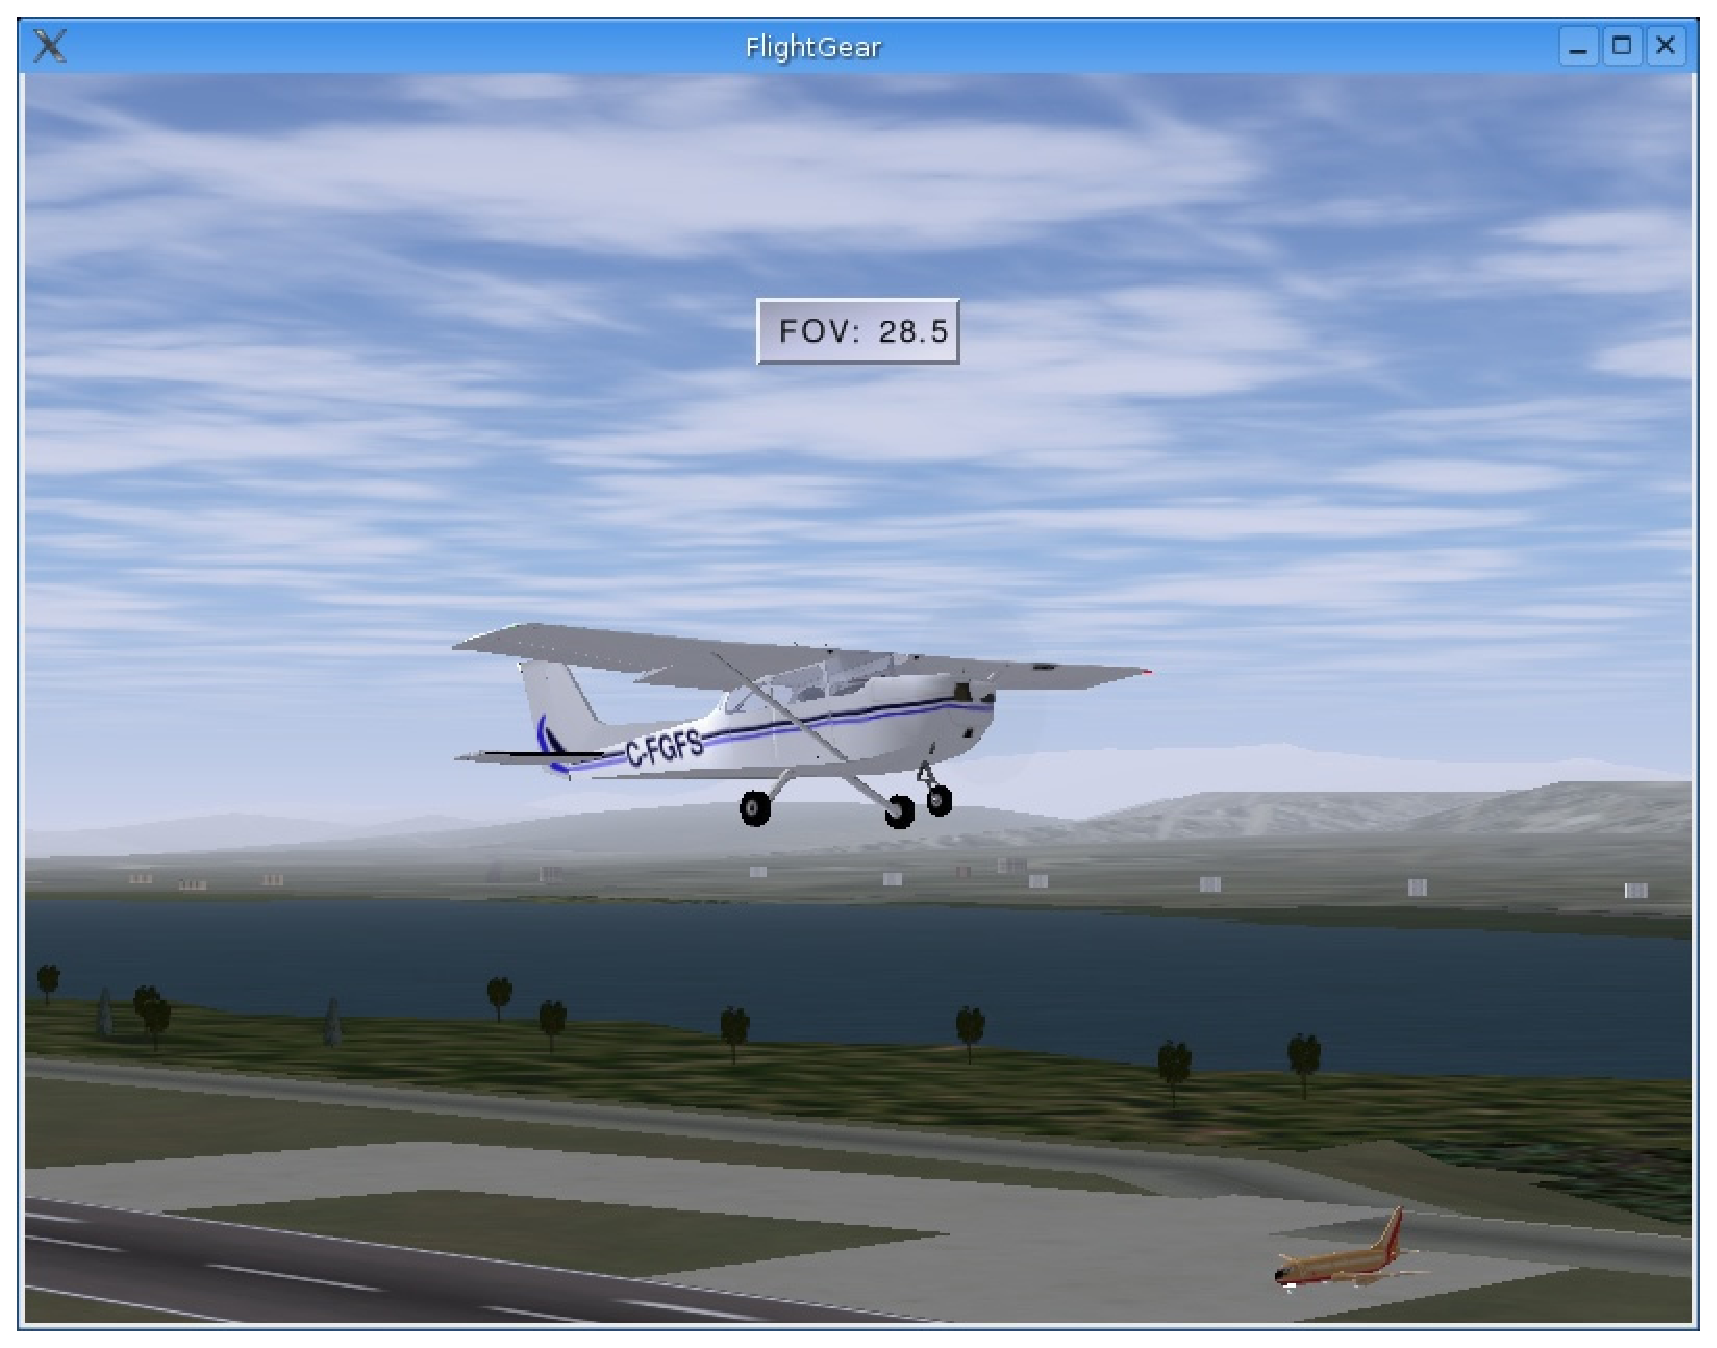
\includegraphics[width=0.5\textwidth]{img/tut_1}
\end{center}
    
You may find the following articles useful if read in conjunction with this
tutorial. They contain many answers to questions that
may arise while reading this tutorial. This first one in paricular is a good
intruction to the airplane's main parts and controls:
\begin{itemize}
	\item \weblong{http://www.gleim.com/aviation/ltf/howtheyfly.php?PHPSESSID=889ab9792636f430a66e3e5d70f7d346}    {http://www.gleim.com/aviation/ltf/howtheyfly.php?PHPSESSID=889ab9792\\636f430a66e3e5d70f7d346}
	\item \weblong{http://www.pilotfriend.com/flight_training/new_site/aerodynamics/aircraft\%20controls.htm}    {http://www.pilotfriend.com/flight\_training/new\_site/aerodynamics/\\aircraft\%20controls.htm}
	\item \web{http://www.flightgear.org/Docs/getstart/getstart.html}
	\item \web{http://en.wikipedia.org/wiki/Aircraft}
	\item \web{http://en.wikipedia.org/wiki/Flight\_controls}
	\item \web{http://en.wikipedia.org/wiki/Airplane\_flight\_mechanics}
	\item \web{http://en.wikipedia.org/wiki/Aircraft\_engine\_controls}
	\item \web{http://www.firstflight.com/flt1.html}
	\item \weblong{http://www.avsim.com/mike/mickey_site/ppilot/ppilot_faq/pp_cessnas.html}{http://www.avsim.com/mike/mickey\_site/ppilot/\\ppilot\_faq/pp\_cessnas.html}
	\item \web{http://www.ig-wilson.com/index.php?f16land}
	\item \web{http://www.navfltsm.addr.com/}
\end{itemize}

This tutorial is accurate to the best of my knowledge, but inevitably will
contain some mistakes. I apologize in advance for any bad habits you may
develop from following this tutorial.
\section{Starting Up}
\label{sec:Hardware}
    
     
On MS Windows, \fg{} has a GUI Wizard that will let you choose what
to fly and where to fly from. First choose the Cessna 172p airplane as shown 
below. To match this tutorial do not choose the 2D panel version. 
(You may however find in the future that the 2D version is more appropriate 
for training) Press the \button{Next} button to choose your airport.


\begin{center}
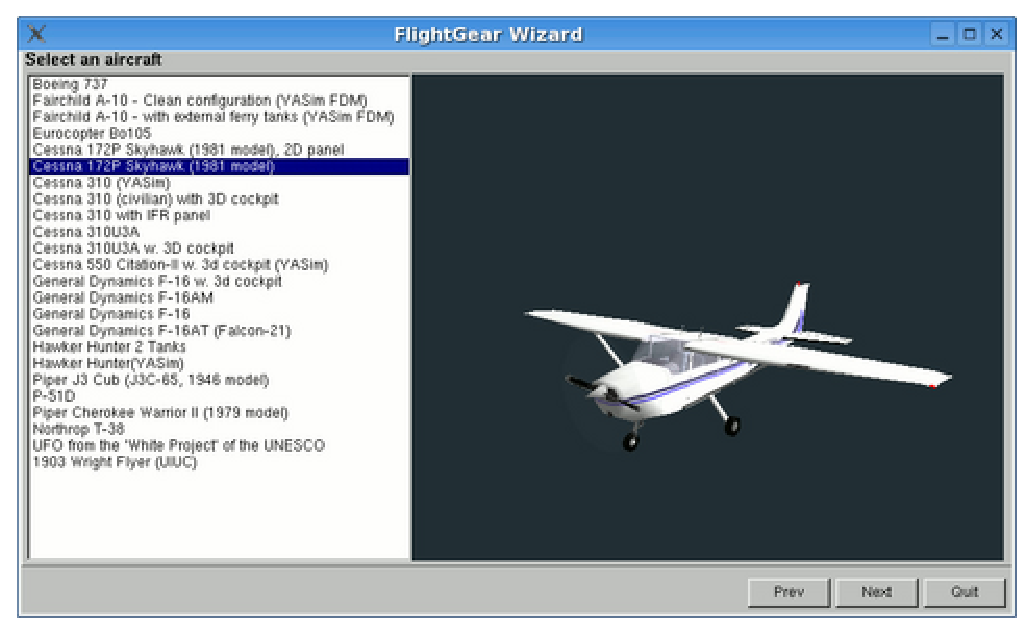
\includegraphics[width=0.5\textwidth]{img/tut_2}
\end{center}
    
You can start from any airport for this tutorial, but I will assume that you 
will start from FlightGear's default airport of San Francisco (KSFO):


\begin{center}
\includegraphics[width=0.5\textwidth]{img/tut_3}
\end{center}

Once you have selected KSFO and pressed the \button{Next} button, you can set
any number of options for the simulator. For your first flight, I suggest
starting at noon. I woul dalso recommend that you start with a small resolution
of $800\times600$. Later on you can play around with the options and use a
higher resolution, but this obviously adversly affects performance.Press the 
\button{Run} button and the \fg{} will start with the options you selected.


\begin{center}
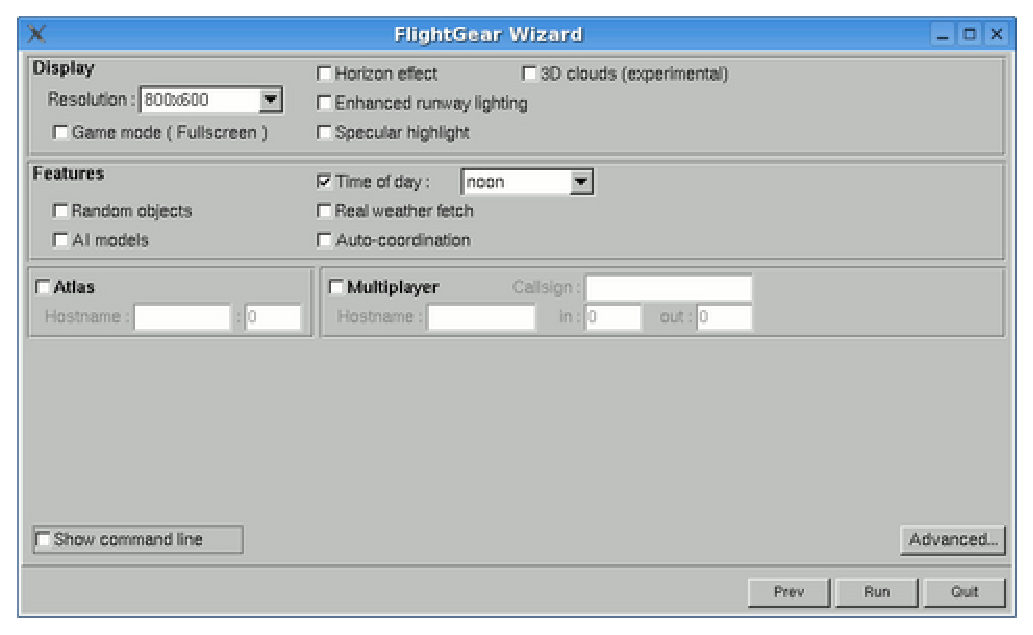
\includegraphics[width=0.5\textwidth]{img/tut_4}
\end{center}

   If you have problems running the latest version FlightGear on
   your Windows system, you may want to try an earlier version with lower
   graphics requirements (for example 0.9.8) You can find previous releases on 
   the FTP mirrors mentioned at the top of the \fg{} download page:
   \weblong{http://www.flightgear.org/Downloads/binary.shtml}.
   
If you are running under Windows Me and the flight simulator suddenly starts
\index{troubles!stuttered simulation}stuttering, with the frame rate dropping, 
try killing all tasks except Explorer and Systray before you
launch FlightGear. If one of the tasks you kill is an antivirus or
such protection software, this is an obvious security risk. Also, on one
Windows Me machine, a \fg{} of $800\times600$ yielded good results,
while a lower resolution of $640\times480$ triggered much lower FPS levels 
(Frames Per Second).)

On Linux and other Unix-like 
systems, you may have to run \fg{} from the command line. If you have
installed \fg{} but cannot find it within your menu system, try the following:

\begin{itemize}
  \item From a terminal window (also named ``console'' window) try
  running the  \command{fgrun} command. If installed, this will run the same 
  cute dialog windows as under Windows.

	\item Alternatively, open a terminal window and type the following command:
  \command{fgfs --timeofday=noon}. If the FlightGear window you get is too 
  small, close it and restart FlightGear with this command: 
  \command{fgfs --timeofday=noon --geometry=1024x768}.
\end{itemize}

Without the \command{--timeofday=noon} option, \fg{} will start at the current
time in San Francisco - often night-time if you are in Europe. To get a 
daytime environment from within the simulator, 
select \button{Weather->Time of Day} from the menu and select \button{Noon}.


\begin{center}
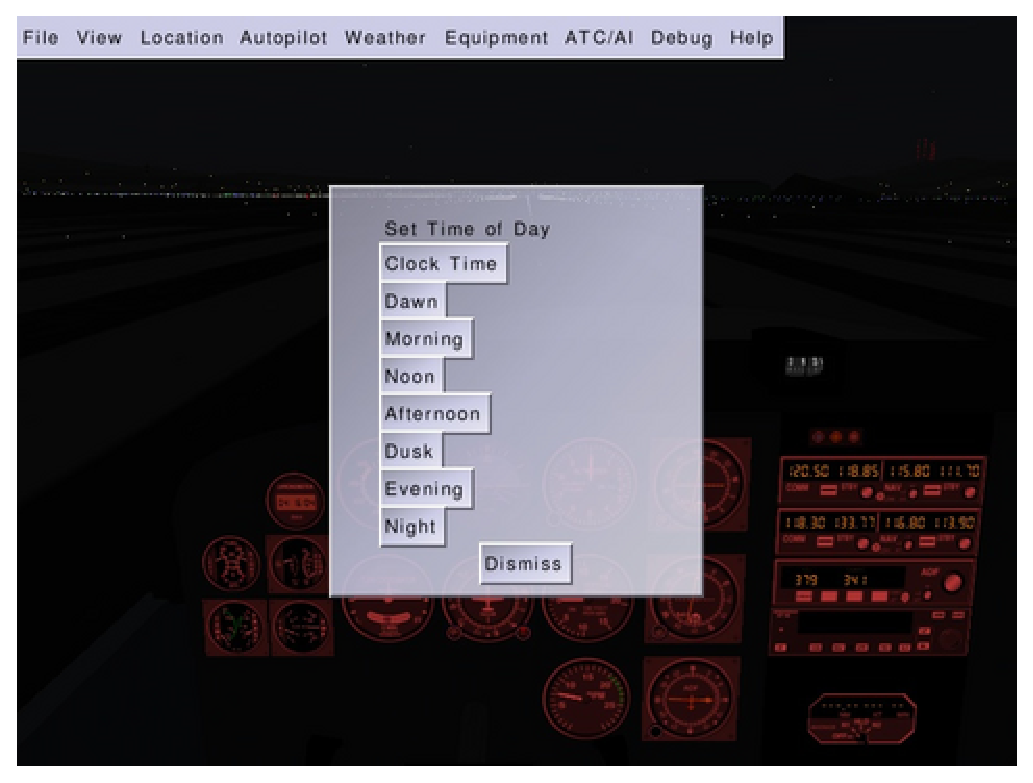
\includegraphics[width=0.5\textwidth]{img/tut_5}
\end{center}


If running \fg{} from a men (e.g. under KDE or Gnome), you can edit the 
FlightGear launch icon properties and change the simple \command{fgfs} fgfs 
command to something like \command{fgfs --timeofday=noon --geometry=1024x768},
or include whatever command options you wish. Further details of the command
line options can be found in Chapter~\ref{takeoff}, 
\textit{Takeoff: How to start the program}.

\section{The First Challenge - Flying Straight}
\label{sec:FlyingStraight}
    
Once \fg{} is started you will see the following window and hear the sound of 
an engine:


\begin{center}
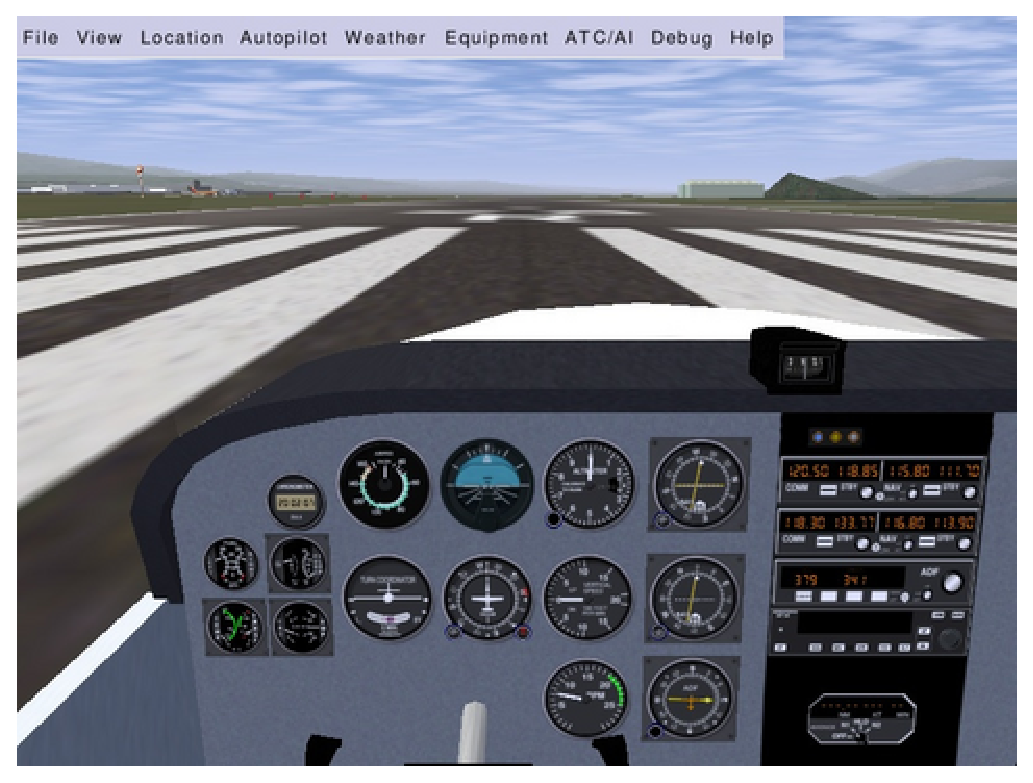
\includegraphics[width=0.5\textwidth]{img/tut_6}
\end{center}

On startup, the aircraft is at the end of the runway with the engine running at
low power. The airplane will ocassionally tremble a little, but it won't move.
    
\subsection*{About the keyboard.}\index{keyboard}
    
\begin{itemize}
	\item In this tutorial, a lowercase key letter indicates you should simply
  press that key. An uppercase means you must press shift and that key. 
  (The \textcolor{blue}{\key{$\Uparrow$~Shift}} keys are those two keys with 
  a hollow fat arrow pointing upwards.) In other words: if you are told to type
  ``v'', simply hit the \key{v} key briefly. 
  \index{keyboard!uppercase and lowercase keys} If you are told to type ``V'', 
  press the \key{Shift} key down and while you have it pushed down, hit the 
  \key{v} key, then release the \key{Shift}  key. (In short: V is the same as 
  \key{Shift-v}.)
	\item The tutorial will assume you have the the \key{NumLock} switched on. 
  \index{keyboard!numeric} When switched on, you should find a small green
  light on at the right of your keyboard. Press the 
  \textcolor{green}{\key{NumLock}}key repeatedly until the lamp is on.
\end{itemize}


\begin{center}
\includegraphics[width=0.5\textwidth]{img/tut_7}
\end{center}

\key{v}\index{view!changing}
Press \key{v}, to view the aircraft from the outside. Type v repeatedly to
scroll through a number of different views until you return to the cockpit.
Typing \key{V} will cycle backwards through the views.):


\begin{center}
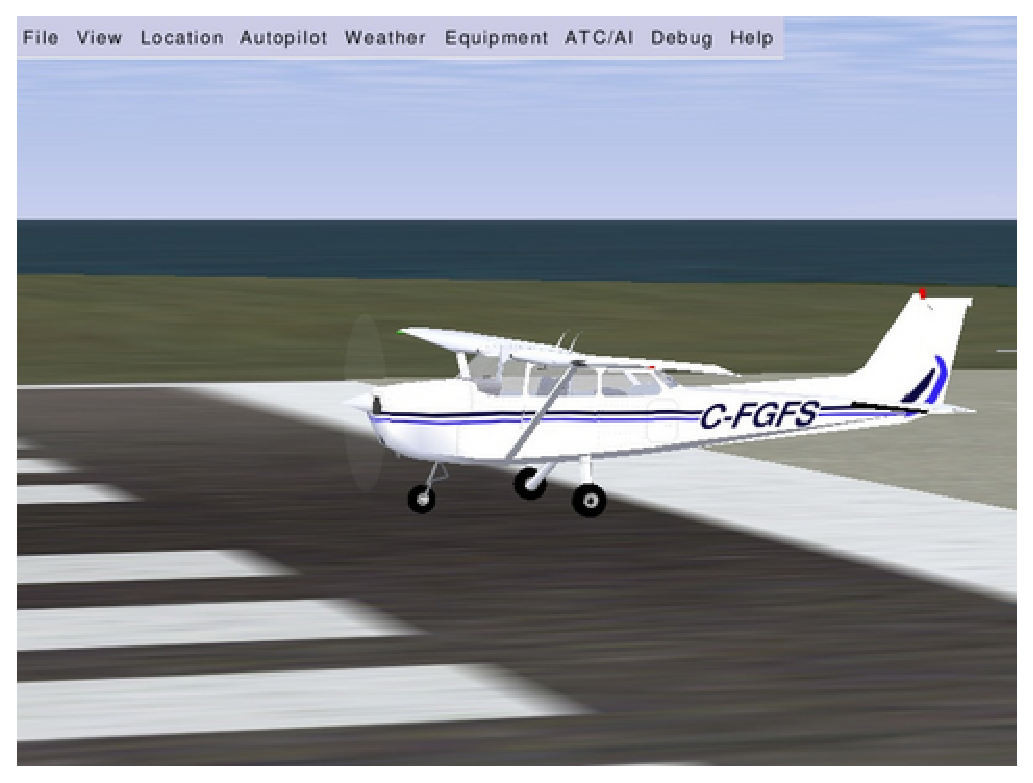
\includegraphics[width=0.5\textwidth]{img/tut_8}
\end{center}

In real life, we would have inspected the airplane all around to check 
everything is working, nothing is hampering the moving parts, 
and nothing is obstructing the instrument openings. In the simulator, this is
already done for us before we start.

Hold the \key{Page Up} key down for eight or so lengthy seconds. You will
hear the engine sound rise.

The airplane will start accelerating down the runway. As it does so, it will 
drift to the left, before finally taking off, banking to the left, 
falling to the ground and crashing. 

\index{view!instant replay}
You can see a replay of the crash using the  \button{View -> Instant Replay}
menu. Click the \button{Replay} button at the bottom of the dialog window, then
use \key{v} and \key{V} to see the airplane from the outside. The
picture below shows the end part of the flight. You can take a snapshot by
typing the \key{F3} key. You can alos use the \key{F10} key to toggle the menu 
bar on or off.


\begin{center}
\includegraphics[width=0.5\textwidth]{img/tut_9}
\end{center}

Having observed your crash, exit from \fg (using \button{File->Quit}) 
and restart the simulator using the same options as before.

In order to fly straight you need the airplane's control\index{yoke}
\weblong{http://en.wikipedia.org/wiki/Yoke_(aircraft)}{yoke}:


\begin{center}
\includegraphics[width=0.5\textwidth]{img/tut_10}
\end{center}

You can control the yoke using a joystick, or by moving the mouse. For this 
you need to be in mouse yoke mode. Get in that mode by clicking the right 
mouse button. The mouse cursor becomes a $+$ sign. Move the mouse and see the 
yoke moving accordingly. Type \key{v} to see the plane from the outside. If you
move the mouse again you will see the tail
\weblong{http://en.wikipedia.org/wiki/Elevator_(aircraft)}{elevator}
and the \weblong{http://en.wikipedia.org/wiki/Aileron}{ailerons}
at both wings ends. If your viewpoint is too far from the aircraft to see the
movement, type \key{x} a few times to zoom in. 
Type \key{X} to zoom back out. \key{Ctrl-x} for default zoom. Type
\key{V} to get back inside the plane.

Clicking the right mouse button again gets you in mouse view mode.
In this mode the mouse cursor will be a $\leftrightarrow$. sign. This allows you
to look around easily. Clicking the left mouse button will re-center the view. 
A further right click will return you to the normal mouse mode.

To summarize, the right mouse button cycles the mouse through three modes:
\begin{itemize}
	\item \textit{Normal mode}\index{mouse!normal mode}. This mode allows you to 
  click on the menu and on the instrument panel.
	\item \textit{Yoke mode}\index{mouse!yoke mode}.\index{yoke!mouse yoke mode} 
  The mouse controls the yoke (+ pointer shape). 
	\item \textit{View mode}\index{mouse!view mode}. The mouse controls the 
  direction you look towards  $\leftrightarrow$) pointer shape).
\end{itemize}

Try taking off again using the mouse to control the yoke. Right-click to put 
the mouse in yoke mode ($+$pointer shape) and raise the engine throttle to 
maximum by holding the \key{Page Up} key down. Do not try to keep the airplane 
rolling straight on the runway using the mouse/yoke. Let it drift leftwards.
Wait till it rises in the air. Then use the mouse to try and get the
airplane to fly straight. (If you want to control the airplane on the
ground see section \ref{sec:TaxiTurning}.)

You will find that you must prevent the airplane from banking to the left:


\begin{center}
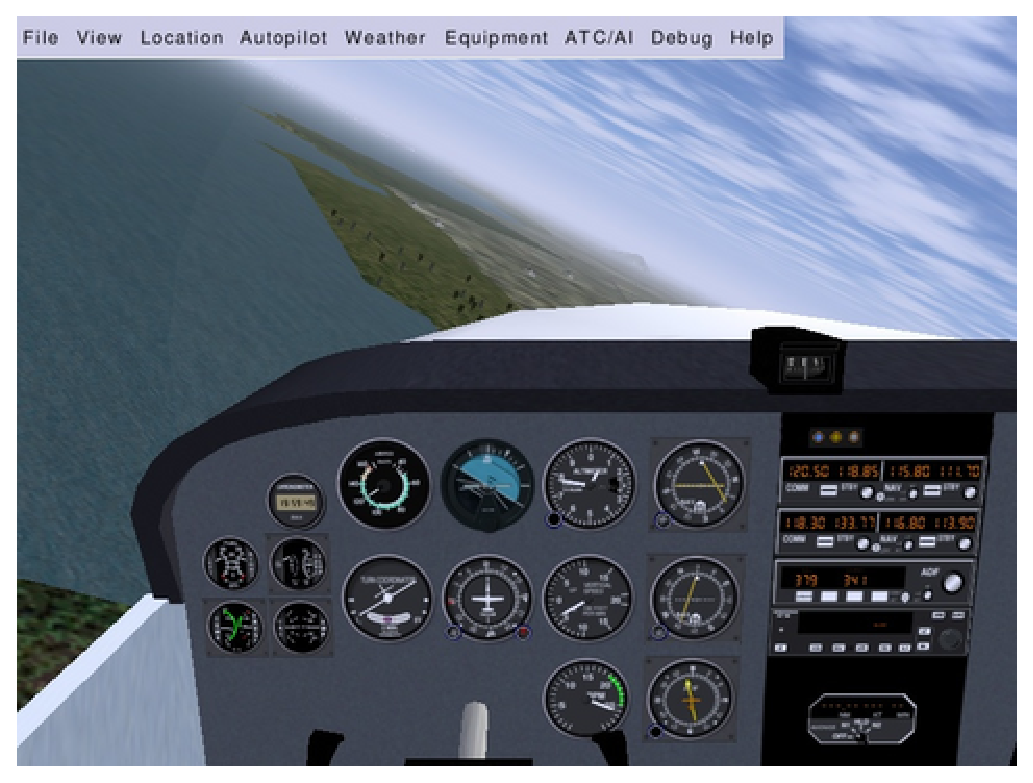
\includegraphics[width=0.5\textwidth]{img/tut_11}
\end{center}

%\pagebreak[4]

Prevent it from banking to the right:


\begin{center}
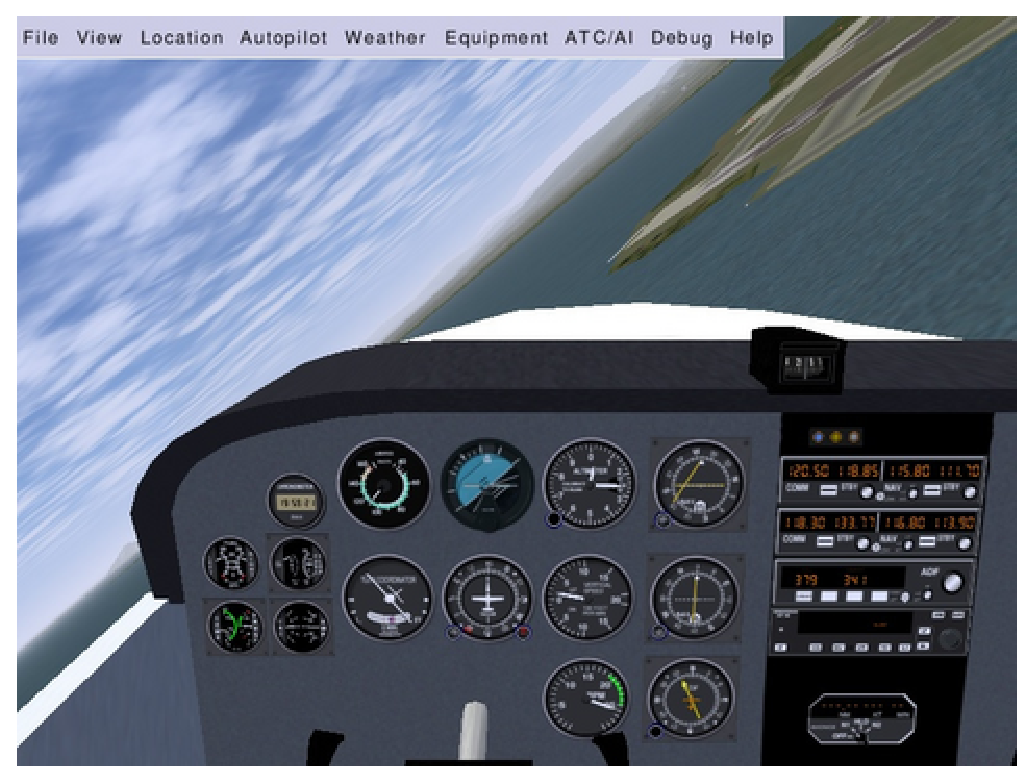
\includegraphics[width=0.5\textwidth]{img/tut_12}
\end{center}

Prevent it from plunging to the ground:


\begin{center}
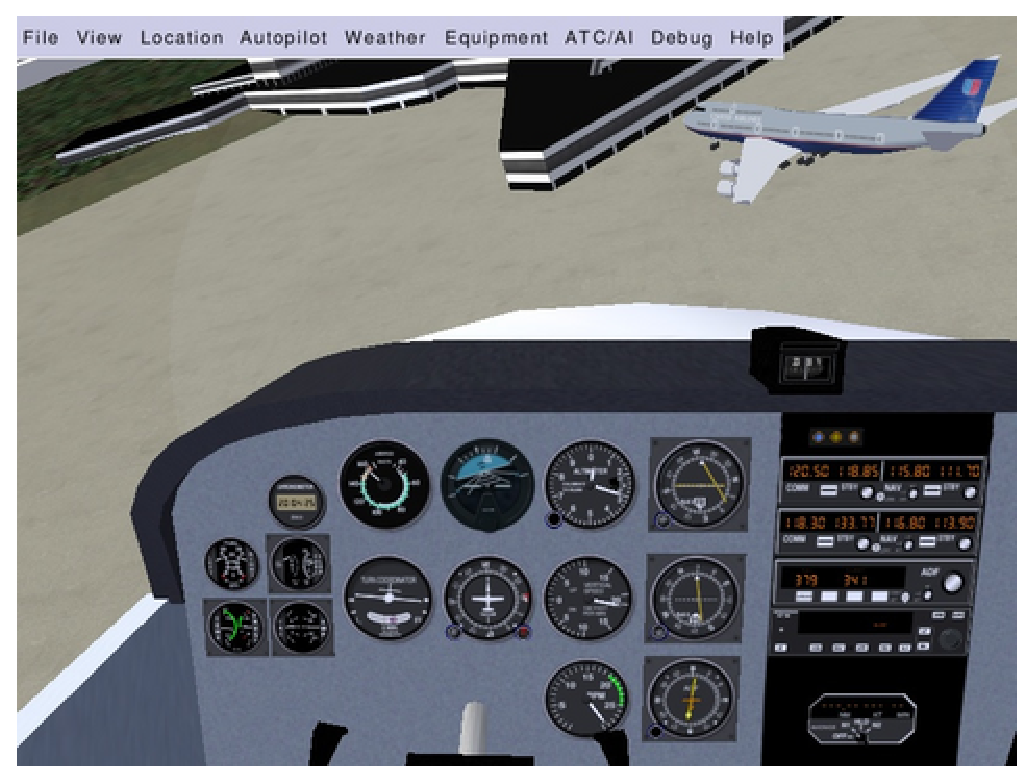
\includegraphics[width=0.5\textwidth]{img/tut_13}
\end{center}

%\pagebreak[4]

Try to fly more or less straight, with the horizon stable above the airplane 
nose:


\begin{center}
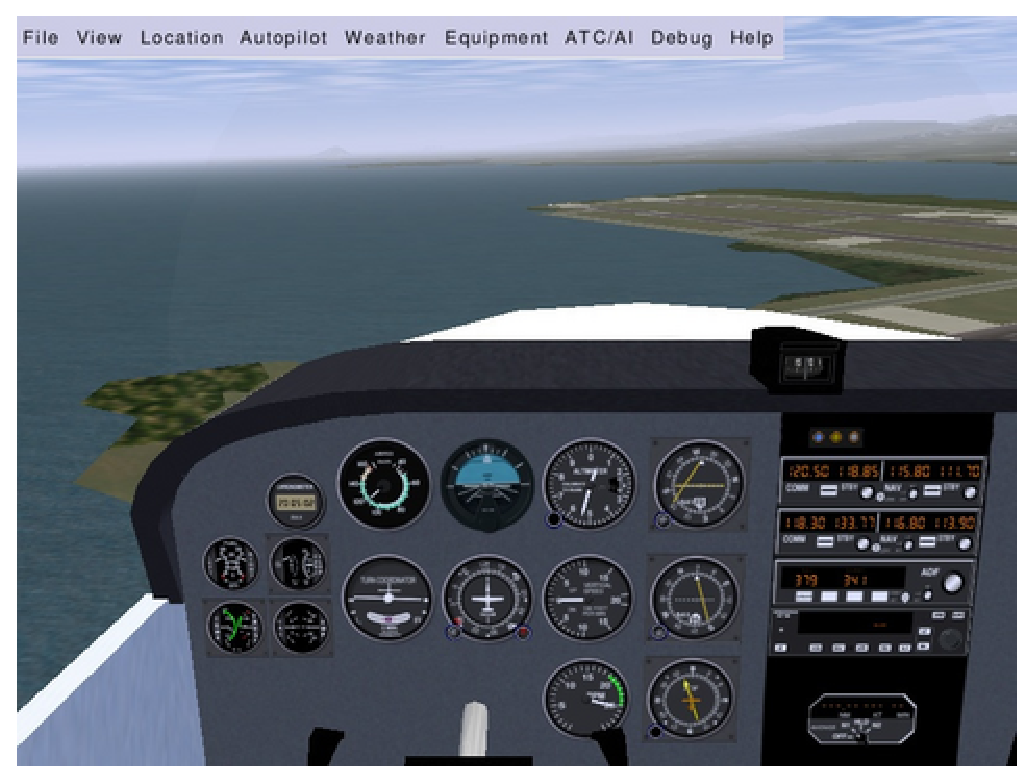
\includegraphics[width=0.5\textwidth]{img/tut_15}
\end{center}

Whatever your skills at video games or simpler simulators, you will probably 
not succeed. The airplane will crash, probably quite soon after take-off.
This is the moment where most candidates get desperate and abandon trying 
to fly a simulator or a real aircraft. Just hold tight and keep trying. 
Eventually you will develop a feel for the control inputs required.

\index{yoke!pulling}
The most common error is moving the mouse forwards to bring the nose up. In
fact, you must pull the yoke by moving the mouse backwards to do this. 

Equally, when you want to lower the airplane's nose, you must move
the mouse forwards. This can seem odd, but all airplane control yokes
are designed that way. With time, you will wonder how you every thought it
worked any other way. \index{troubles!mouse speed} You will also find that 
small mouse movements have a large effect on the aircraft. You may find that
decreasing your mouse sensitivity may help initially.

If you have difficulty visualising this, the following analogy may help.
Imagine a soccer ball is on your desk and you have ``glued'' your hand 
to the top of it. If you move your hand forwards the ball will roll forwards 
and your fingers will point to to the desk. If you move your hand backwards the 
ball will roll  back and your fingers will now point up at the ceiling. 
Your hand is the airplane:


\begin{center}
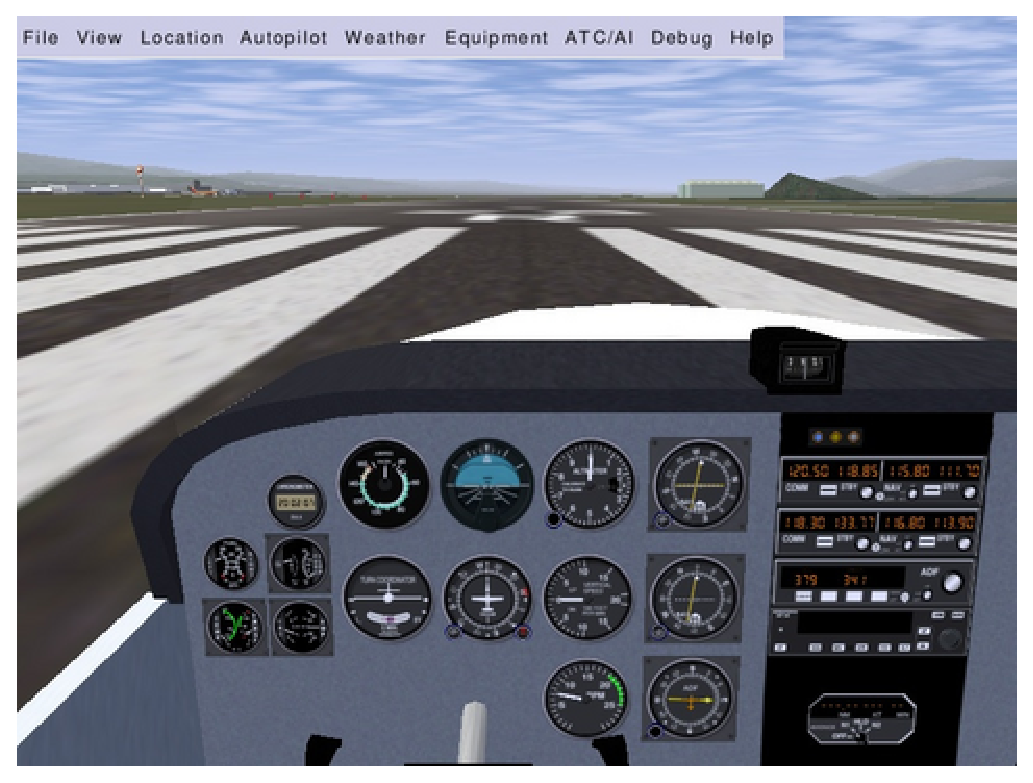
\includegraphics[width=0.5\textwidth]{img/tut_6}
\end{center}

Another common error is the assumption that the control inputs directly
match airplane bank. In other words, you believe if the control yoke is
level, the airplane will fly level. This is false. Actually the yoke
bank controls the speed at which the airplane banks. If the airplane is
banked 20$\textdegree$ to the left and the control yoke is level, the
airplane will stay banked at 20$\textdegree$ left until some other force
affects it. If you want to return the airplane to level flight, you have to
turn the control yoke slightly to the right (move the mouse slightly
rightwards) and keep it slightly to the right for a while. The airplane
will turn slowly rightwards. Once it is level with the horizon, bring the
control yoke level too. Then the airplane will stay level (until some other
force changes its orientation).

A third error is trying to find ``the right position'' for the
yoke/mouse. Naturally, you will want to find the fine tuning that will leave 
the airplane fly straight. Actually there is no such ideal yoke
position. The airplane is inherintely unstable in the air. You must constantly 
correct the airplane's attitude and keep it flying straight with tiny movements
of the mouse. This may seem to take all your concentration intially,
but just like driving a car, keeping the aircraft straight and level will
become second nature. You can also use the to keep the airplane level
during long flights.

A key helper in making the small adjustments is to keep your eyes on the outside
scenery and not get fixated on the instruments or the yoke. Check the angle of 
the horizon and its height above the airplane's nose. The horizon line and the
airplane engine cover are your main flight instruments. Look at
the instrument panel only once in a while.

While the mouse is in yoke\index{yoke!mouse yoke mode} control mode
($+$ pointer shape), don't move it close to the FlightGear window
edges. Once the mouse leaves the window, it stops controlling the aircraft.
If you want to get the mouse outside of the window, first go back to standard 
mouse mode by clicking two times on the right mouse button.

You can also control the yoke using the four \key{keyboard arrow} keys
or the keypad \key{8}, \key{2}, \key{4} and \key{6} keys. While initially this
may seem easier than the mouse, you cannot make the very fine adjustments
required for accurate flying.

You may hear beeping sounds while flying around the airport. Those are
landing aid signals\index{landing!aid signals}. Don't worry about them for the
moment - they aren't warning your of danger.

You will know that you have mastered this when you can make the aircraft climb
steadily in the air. The next step is to learn to keep the aircraft at a constant
altitude, or to make it ascend or descend slowly and under your control.

Keeping the aircraft at a constant altitude involves observing the altimeter
and making small changes with the mouse forwards or backwards to stop the 
aircraft ascending or descending respectively.

\index{altimeter} The altimeter instrument is at the middle top of the 
instrument panel. The long needle shows hundreds of feet, the short needle 
shows thousands of feet. The altimeter below shows an altitude of
300 feet, approximately 100 meters.


\begin{center}
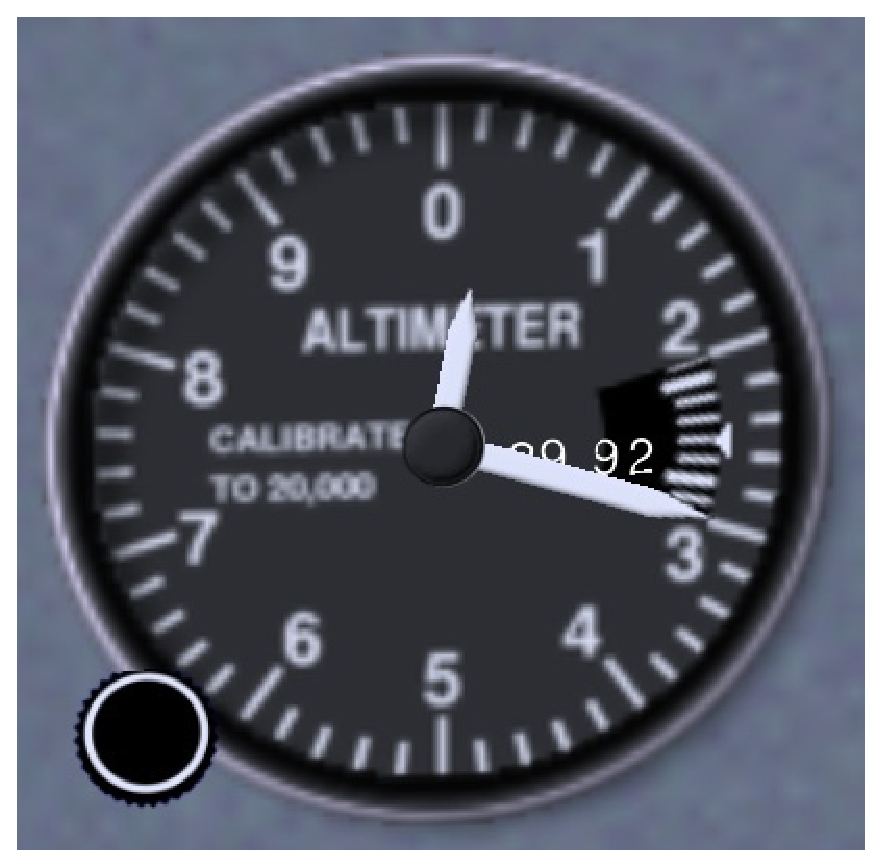
\includegraphics[width=0.25\textwidth]{img/tut_17}
\end{center}

As you ascend or descend the altimeter will change accordingly, turning 
anti-clockwise as you descend, and clockwise as you gain height. If you see
the altimeter ``unwinding'' you will be able to tell that you are losing height
and move the mouse backwards slightly to raise the nose.
After a while you will notice that when flying level the nose of the aircraft
is always in the same position relative to the horizon. This is the aircraft
attitude for level flight. By putting the nose in that same position, you will
achieve almost level flight without having to reference the instruments. From
there you can fine-tune your altitude.

Beware: an altimeter does not automatically show the absolute altitude
above sea level\index{altitude!absolute}. You must adjust for the local air
pressive. The little black knob on the lower left side of the
altimeter\index{altimeter!tuning} allows you to adjust the altimeter. Start 
\fg{} and stay on the ground. Click (in normal mouse mode) inside the black knob. 
A click on the left half makes the altimeter turn back. On the right half the 
altimeter turns forward. Use that little knob to tune in the curraent altitude. 
The principle is you use the knob when you are sure about the altitude. If
you know you are at 1,100 feet altitude, tune in 1,100 feet on the
altimeter. Clicking with the middle mouse button makes the knob
turn faster. Type \key{Ctrl}-\key{c} to see the two button halves
highlighted.

To make settings the altimeter easier, airports advertise their altitude in 
various ways. They may provide a radio service (called ATIS in the USA) 
to broadcast the current air pressure at sea level. This is expressed in 
inches of mercury. The altimeter contains a small scale inside which is
calibrated in this way. You can set your altimeter using this scale. 
Alternatively, if you are on the ground and know the altitude of the airport,
you can simply adjust your altimeter until it displays the correct altitude.

\vfill


\begin{center}
\includegraphics[width=0.25\textwidth]{img/tut_18}
\end{center}

Note that there is an important difference between ``altitude above sea 
level'' and ``altitude above the ground''. If you fly near Mount Everest at an
altitude of 24,000 feet above sea level (AMSL), your altitude above the ground 
(AGL) will be much less. Knowing the altitude of the ground around you is 
obviously useful.

    \section{Basic Turns}
    \label{sec:InFlightTurning}

Once you are able to fly straight, even just approximately, you can begin to 
learn to turn. The principle is simple: 
\begin{itemize}
	\item When the airplane is banked to the left, it turns to the left.
  \item When the airplane is banked to the right, it turns to the right.
\end{itemize}


\begin{center}
\includegraphics[width=0.25\textwidth]{img/tut_19}
\end{center}
\index{turn coordinator}

\index{turn coordinator} To turn, you do not need high levels of bank. 
20$\textdegree$ is a good level of bank to get a safe and steady turn. This it 
what the turn coordinator is used for. On the picture below the indicator shows 
the airplane is banked 20$\textdegree$ to the right. This is just right. You
can also tell the bank angle by observing the angle of the horizon.
   
Try the following: keep the airplane banked around those 20$\textdegree$ for a 
few minutes and look at the ground outside the aircraft You will see the same 
ground features appear again and again, every 120 seconds. This shows you 
need 120 seconds to make a 360$\textdegree$ turn (or 60 seconds for a 
180$\textdegree$)turn). This is particularly important when navigating.
Whatever speed the airplane is flying, if you bank at 20� you always need 60 
seconds to make a 180� turn in the c172p.
      
So, by banking the airplane to the left or to the right, you make it turn to 
the left or to the right. Keeping the airplane level with the horizon keeps 
it flying straight. The little purple ball in the bottom of the turn indicator 
shows the sideways forces. If you turn neatly (using the rudder a little bit), 
the ball will remain centered. If the ball is pushed say rightwards, this 
means you the pilot too are pushed rightwards. Like in a car turning to the 
left. During a neat turn in an airplane, even a strong turn, the passengers 
never endure a sideways force. They are only pushed a little harder on their 
seats by the centrifugal force.

By experimenting you will notice you easily get fast and spectacular turns by 
banking the airplane to high angles and pulling on the yoke. It would be mad 
to do this with a real airplane if you are a beginner or if you have passengers 
aboard. However, part of real life training is making turns at up to a 
60$\textdegree$ bank angle. 
      
      
\section{Taxiing on the ground}
\label{sec:TaxiTurning}
    
The picture below shows the \index{tachometer} instrument. It displays how fast 
the engine is turning in hundreds of revolutions per minute (RPM).


\begin{center}
\includegraphics[width=0.25\textwidth]{img/tut_20}
\end{center}

Type the \key{Page Up}  key a few times,
until the tachometer is showing 1,000 RPM (as shown above). If required
type the \key{Page Down} key to decrease the engine speed.

At roughly 1,000 RPM, the airplane will move forward on the runway, but it will 
not accelerate nor take off.

\index{brakes!right wheel [.] (dot)} Type the ``\key{.}''key (\key{Shift-;} on 
Azerty keyboards). The airplane will make a sharp turn to the right. If you 
keep the ``\key{.}''key down the airplane will halt. When you type the 
``\key{.}'' key, you activate the brake on the right wheel of the airplane. 
That makes the airplane turn right and eventually halt.

\index{brakes!left wheel [,] (colon)} To activate the brake on the left 
wheel, use the ``\key{,}'' key. 

\index{brakes} The ``\key{,}'' and ``\key{.}''  keys simulate two brake pedals 
located at your feet on a real airplane. Using the throttle and the brake pedals
you can fontrol the speed of the aircraft and cause it to turn on the ground. 

The brakes can be very useful when taxiing slowly on the runway. You can also
steer the nosewheel of the aircraft. In a real airplane this is done by pushing
the rudder pedals with your feet. You push with your feet on the side you want 
to turn towards. If you don't have real rudder pedals, there are two ways to 
control the virtual rudder pedals:
\begin{itemize}
	\item Using the keypad  \key{0} and \key{Enter}keys 
  \index{rudder!keyboard control}. If you type the keypad \key{Enter} key say 
  seven times, you will see the airplane firmly turns to the right and 
  stays turning that way. Type the keypad \key{0} key seven times to get the 
  airplane back rolling (almost) straight.
	\item Using the mouse. While the mouse is in yoke control mode 
  ($+$pointer shape), if you hold the left mouse button down, the mouse controls 
  the rudder\index{mouse!rudder control} \index{rudder!mouse control} instead 
  of the yoke. This method is much more precise.
\end{itemize}
 
Start the simulator, Type \key{v} or \key{V} to view the airplane from
the outside and keep \key{x} down a couple of seconds to zoom in on the
airplane. Look at the front wheel and keep keypad \key{0} down. Then
keep keypad \key{Enter} down. See the front wheel turn. Click on the
right mouse button to get in yoke control mode ($+$ pointer shape).
Keep the left mouse button down to get in rudder control mode and move
the mouse to the left and to the right. Note that the rudder, that big
vertical control surface at the rear of the plane, moves together with
the front wheel.

I tend to control the rudder pedals using the mouse while the front
wheel is on the ground and use the keypad \key{0} and \key{Enter}
keys once it has lifter off. In other words: I
keep the left mouse button down while the front wheel is on the
ground. This allows for a precise and easy rudder control on the
ground. Then I simply release the left mouse button once the front wheel 
lifts off. 


\begin{center}
\includegraphics[width=0.5\textwidth]{img/tut_23}
\end{center}

This is the airspeed indicator (ASI), calibrate in nautical
miles per hour (knots).


\begin{center}
\includegraphics[width=0.25\textwidth]{img/tut_24}
\end{center}

A knot\index{speed!units!knot [nautical mile per hour]} is 1.85325
kilometer/hour. So, if you want to have a rough idea of your speed in
flight expressed in km/h, multiply the knots displayed by 2. A knot is
1.15115 miles per hour, so very roughly, 1 knot is 1 mph. Note that some
aircraft ASIs (in particular the Piper J3 Cub) display mph instead of knots.

Note the airspeed indicator displays the speed of the aircraft compared
to the surrounding air, not the speed compared to the ground like a car
speed indicator does. If the plane is halted on the ground and there is
a 10 knot wind blowing towards its face, the airspeed indicator will
display 10 knots airspeed, although the plane will not move.

When the airplane rolls over the runway at more than 40 knots, you must
prevent the front wheel from touching the ground. During take off, once
over 40 knots you can make the front wheel leave the ground by pulling back
a little bit on the control yoke. Don't turn sharply at high speed on the ground. Otherwise you may cause the
aircraft to tip over. 

The picture below shows the front wheel slightly lifted. Don't overdo
this. Keep the airplane's white nose cover well below the horizon. You
just need to lift the plane's nose very slightly.


\begin{center}
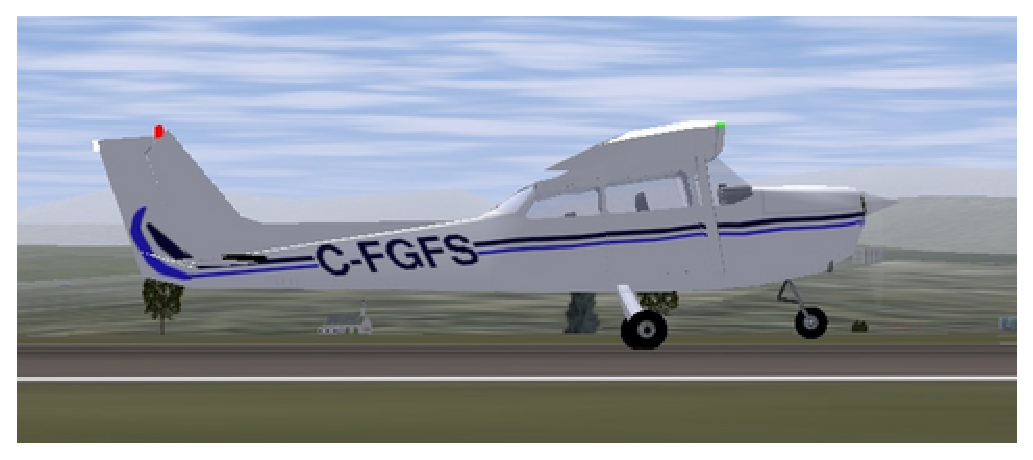
\includegraphics[width=0.5\textwidth]{img/tut_25}
\end{center}

The reason why you must raise the front wheel is it is not designed to
roll at high speeds. It would shimmy and wear out.

Question: if the front wheel no longer touches the runway, how do you
steer the airplane? Answer: still using the rudder pedals. The
rudder pedals are also linked to the tail rudder, that big vertical moving
part at the tail of the plane:


\begin{center}
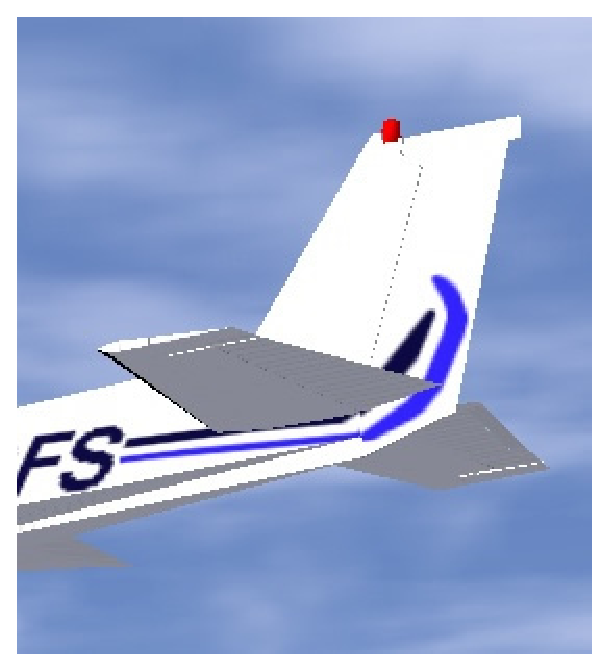
\includegraphics[width=0.5\textwidth]{img/tut_26}
\end{center}

At air speeds above 40 knots, the rudder is adequate to steer the airplane. 

The rudder pedals command both the front wheel and the rudder at the
airplane's tail. So, just move the rudder pedals...

Note the front wheel and the tail rudder don't make the airplane turn
exactly the same way. So when the rudder takes over the front wheel,
you must adapt the rudder pedals angle. That means fast typing keypad
\key{0} and keypad \key{Enter} (or hold the left mouse button down and
tightly control the rudder with the mouse).

Once you've become familiar with this, you will be able to keep the airplane 
straight on the runway during take-off.

Say the airplane is heading too much to the right. You type
keypad \key{0} a few times to make it turn back to the left. Don't
wait till the trajectory is corrected. Type keypad \key{Enter} before
the aircraft reaches the direction you wish to travel. Otherwise you will
find that you will over-correct. If you use the mouse, things are
much easier and more precise.

To summarise: two methods exist to steer the airplane on the ground: the
differential brakes on the side wheels and the rudder pedals. This 
control redundancy is very common in aviation. If one method fails, 
you still have another method available as an alternative way to perform 
the task. 

You may be wondering why the aircraft drifts to the left when it rolls on the 
ground, forcing your to compensate with a little push on the right rudder 
pedal? The main reason is the flow of air produced by the propeller. It 
blows along the airplane body, but also corkscrews around the airplane 
fuselage. The upper part of that slight vortex pushes the vertical tail 
to the right. This causes makes the front of the aircraft to head to the left.

You can center all yoke and rudder controls by typing \key{5} on the
keypad. This is a good preflight precaution. Sometimes it can ``save
your life'' in flight. 

\section{Turning in the air}
\label{sec:Turning}
    
As with turning on the ground, there are two methods of turning in the air. 
You can use the wing ailerons (steered by the yoke/mouse) or
you can use the tail rudder (steered by the rudder pedals / the
keypad keys /\key{0} and \key{Enter}.
    
Why these two ways? Partially for redundancy, but mainly because they are 
complementary. The main effect of the rudder is yaw, while the main effect
of the ailerons is roll.
    
\begin{itemize}
	\item When flying close to the ground, it is better not to bank the 
  airplane in order to turn. The rudder is used more instead. Acting on the 
  rudder pedals allows you to turn the airplane without excessive banking. 
	\item When the plane is close above the runway, the two side wheels need to 
  be at the same height above the runway for landing. That means the wings 
  must be level with the horizon. The plane is not allowed to bank. You keep 
  the plane wings level with the horizon by using the yoke/mouse/ailerons. 
  Note this does not need to be perfect. A bank of a few degrees is harmless.
	\item In flight, especially at high speed, the rudder is a dirty way to make 
  the airplane turn: 
\begin{itemize}
	\item It causes the airplane to present its flank to the airstream, increasing
  drag.. 
	\item The airplane will turn very slowly.
	\item You won't have very good control on the turn.
	\item At high flight speed the centrifugal force will be disturbing or even 
  dangerous.
\end{itemize}
Using the yoke/mouse/ailerons allows for efficient, fast, reliable and 
comfortable turns.
  \item The rudder can be vital when the wings are stalled. Indeed, during a 
  stall the wing ailerons become less effective or even useless. 
  (Note that some airplanes can go in a very dangerous stall if you overdo the 
  rudder control at low speed.)
\end{itemize}

When you turn in flight, using the ailerons, you still need the rudder 
a little bit. You add a little bit of rudder. This allows you to 
perfectly compensate for the adverse yaw created when you roll using the 
ailerons. In a real aircraft, you can feel this sideways motion. In the
simulator, you can check this visually on the turn coordinator. In the 
picture below the little ball is pushed rightwards during a strong turn 
to the right using the ailerons. That means you the pilot endure a rightwards 
force too. You can compensate this by pushing the right rudder pedal 
(type the keypad \key{Enter} key a few times). In normal flight you use the 
rudder to keep the little ball centered. 


\begin{center}
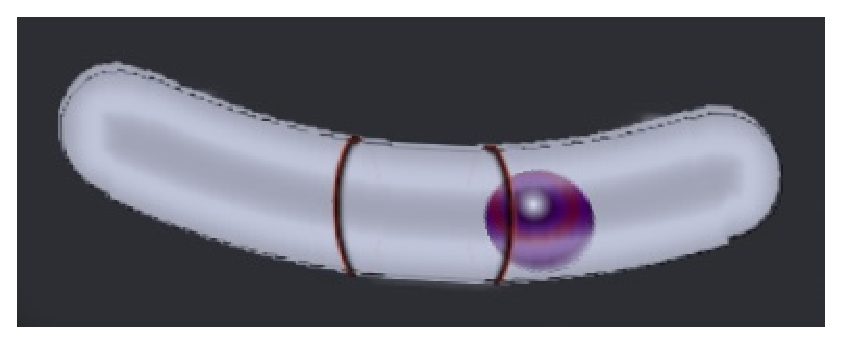
\includegraphics[width=0.25\textwidth]{img/tut_27}
\end{center}
  
So, you tend to turn by using the ailerons in normal flight and by using 
the rudder when close above the ground at low speed. Yet one method never 
completely cancels out the other. You still need the rudder at high altitudes 
and speeds. Reciprocally you have to use the ailerons a little bit when close 
to the ground, to keep the wings level with the horizon. 

Even when taxiing, you should use the ailerons. Otherwise, strong winds can
blow the aircraft onto its side. To counteract this, your should turn the
ailerons into the wind.

It is best never make quick and strong movements with the rudder. On the
ground at high speed this can make the airplane turn to sharply. In flight
at low speed it can cause a very dangerous stall. In flight at high
speed it can cause all kinds of aerodynamic and physical discomfort.
Instead, make gentle movements of the rudder. 

I recommend you train to turn with the rudder in flight. Fly at a low
speed of about 70 knots. Try to keep the altitude stable by increasing
and decreasing the engine power. Use the rudder to turn towards a ground
feature and maintain a heading, then turn the aircraft towards a new heading.
See how the plane yaws. Learn to anticipate rudder
control. Don't try to make steep turns. Use the yoke/ailerons to keep
the wings level constantly.
  
\section{A Bit of Wieheisterology} 
  
Wieheisterology comes from the German phrase ``Wie hei\ss t Er'' -- 
``What's that name''. This section is about gauges, switches and controls of 
the aircraft. It's like the buttons of a video game control pad: you can play 
a game with just the arrow buttons but if you want to get the fun out of the 
game and beat serious opponents you need to learn the functions of the other 
buttons. Equally, in the simulator, you can take off and land a basic airplane 
with just the engine throttle and the yoke but you need all the controls to 
perform securely and efficiently. You need to have at least a basic 
understanding of the physics behind the controls. In emergency situations you 
have to understand how the controls work to be able to cope with their 
deficiencies.

\subsection{Engine control}
\label{sec:EngineControl}
    
An airplane engine is a technological wonder. It is the most powerful, 
efficient, lightweight and reliable fuel energy plant commonly available.

On the bottom left, below the instrument panel you will find the 
\Index{magneto} switch and engine starter:


\begin{center}
\includegraphics[width=0.25\textwidth]{img/tut_28}
\end{center}

To see the switch, either type  \key{P} to get the schematic instrument
panel or type \key{Shift-x} to zoom out (\key{x} or \key{Ctrl-x} to
zoom back in).

You can move the switch with the \key{\{} and \key{\}} keys (use the \key{Alt
Gr} key on Azerty keyboards).

You are probably aware that the fuel inside a car engine is ignited by 
electric sparks. Modern car engines use electronic ignition. An airplane engine 
uses a more old-fashioned (but more reliable) magneto ignition instead. For
redundancy, it contains two such magnetos: the ``left'' one and the ``right'' 
one. When you cahnge the magneto switch on OFF, both magnetos are switched off
and the engine will not run. With the magneto switch on L you are using the 
left magneto. On R you are using the right magneto. On BOTH you use both. 
In flight you will use BOTH.

Given that you use both magnetos in flight, why have the switch? The reason
is that during your pre-flight checks you will verify that each of the magnetos
is working correctly. To do this, increase the RPM to about 1500 then switch 
the magneto switch to L and observe the tachometer. You should observe a 
slight drop in RPM. If the engine cuts out, the left magneto is broken. If 
you do not see an RPM drop, then the switch may be faulty, as both magnetos 
are still switched on. You can then perform the same test on the right magneto.
Of course, in the simulator, the magnetos are unlikely to fail!

Should one of the two magnetos fail in flight, the other one will keep doing 
the job. The failure of one magneto is rare, the failure of both together is 
almost unheard of.

You may have typed \key{\{} to shut the engine down. To start
the engine again after doing so, type \key{\}} three
times in order to put the magneto switch on BOTH. Then use the starter motor
by pressing the \key{Space Bar} for a few seconds, till the engine is started.

You can also turn the magneto switch and start the engine by clicking
left and right of the switch in normal mouse mod). Type \key{Ctrl-c} to
see the two click sides highlighted by yellow rectangles.

If you turn the switch to OFF, the engine noise stops. If you quickly
turn the switch back to L, the engine starts again, though you didn't
turn the switch to START. The reason is the propeller was still
rotating. You should have waited till the propeller came to a halt.
Then, placing the switch on L, R or BOTH won't start the engine. (Once
the engine is halted, always place the magneto switch to OFF.)

\subsection*{The throttle}\index{throttle lever}



\begin{center}
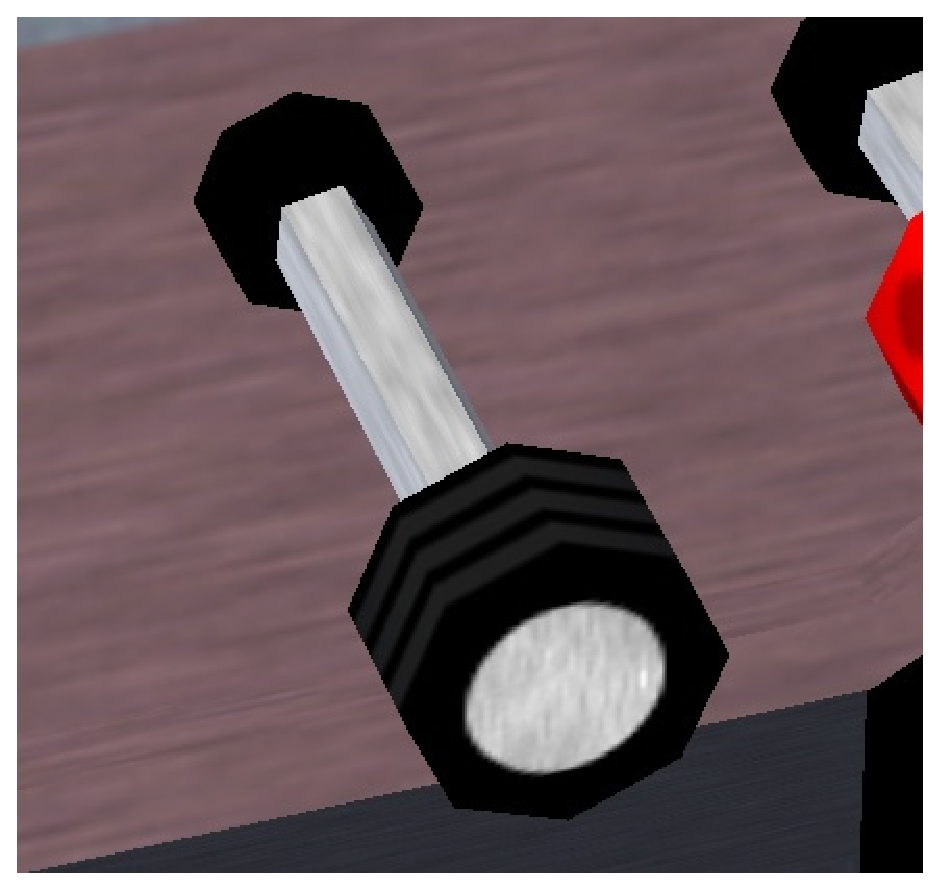
\includegraphics[width=0.25\textwidth]{img/tut_29}
\end{center}

You already know that you increase the engine power by pushing that throttle
lever in (\key{Page Up} key). You decrease the power by pulling the
lever out (\key{Page Down} key). You can also click left and right of
the lever (middle mouse button for quicker moves, \key{Ctrl-c} to
highlight the left and right halves).

What does ``increase the power'' actually mean? Does it mean you increase 
the amount of fuel delivered to the engine? Yes, but this is not enough to 
fully understand what you are doing. You need to be aware that the engine is
also fed with a huge amount of air. The engine's cylinders burn an
\Index{mixture} of fuel and air. Fuel alone wouldn't burn.
Only a mixture of fuel and air can detonate and move the engine
pistons. So when you push the throttle in, you increase both the fuel
and the air fed to the engine.

The amount of air compared to the amount of fuel is critical. The
proportion of the two has to be tuned closely. This is the purpose of
the mixture lever. The picture below displays the mixture lever, pulled out far
too much.


\begin{center}
\includegraphics[width=0.25\textwidth]{img/tut_30}
\end{center}

When the \index{mixture!lever} mixture lever is fully pushed in, you
feed the engine with an lots of fuel and little air. This is known as a 
``rich'' mixture. When the lever is pulled out completely, there is an 
excess of air, known as a ``lean'' mixture. The correct position to produce 
maximum power is in between these two extremes, usually quite close to fully 
pushed in.

When you start the engine and when you take off, you need a fuel-rich
mixture. That means the mixture lever pushed in. A fuel-rich mixture
allows the engine to start easily. It also makes the engine a little
more reliable. The drawback is that a part of the fuel is not burned
inside the engine. It is simply spilled away. This makes the engine
more polluting, it decreases the energy the engine can deliver and it
slowly degrades the engine by causing deposits of residues inside the
cylinders.\index{mixture!optimalisation}

Once in stable flight, you have to pull the mixture lever a little, to
get the optimal mixture. Check this out by doing the following. Start
the simulator. Put the parking brakes on with key B (that is
\key{Shift-b}). Push the throttle in to its maximum. The engine RPM are
now close to the maximum. Slowly pull on the mixture lever (using the
mouse in normal pointer mode). You will see the RPM increases a little.
You get more power, without increasing the fuel intake. You spill no
more fuel in the engine and it pollutes less. If you continue to pull
the mixture lever, the RPM will decrease back away, because now there
is too much air. The excess of air slows the explosions down inside the
cylinders and decreases the explosion temperature, hence the
thermodynamic yield decreases. You have to tune in the optimal mixture. For
thermodynamic reasons, the best mixture isn't exactly at maximum power - it
is better for the engine to be running very slight richer or leaner than
maximum power. You can find the maximum power point by the fact you get the
highest RPM. (Another method is to check the engine exhaust
temperature. Roughly, this is the point at which you get the highest temperature.)

The mixture control allows you to burn less fuel for the same speed and 
distance, and therefore fly farther and pollute less. It can also cause 
serious trouble. Suppose you go flying at high altitude and pull on the 
mixture lever accordingly. Then you descend back in order to land. 
If you forget to push the mixture lever in, The fuel/air mixture will become 
far too lean and the engine will simply halt. You may think the engine is 
failing and panic, while you only have to push the mixture lever back in\ldots

When landing, you have to tune back in a mixture that is a little too
rich in fuel. This means pushing the mixture lever in. That way the
engine becomes a little more reliable and will be better adapted to a
decrease in altitude.

I wrote above that placing the magneto on OFF is not the right way to
stop the engine. The right method is to pull the mixture
level\index{engine!right method to switch off}. First pull the throttle
out completely, to get the engine to minimum power and fuel
consumption. Then pull the mixture lever, till the engine stops because
the mixture contains too much air. This ensures the engine doesn't get
poised by spilled fuel residues. Finally, turn the magneto switch to
OFF to ensure the engine won't start back accidentally.

An important warning: you may think the RPM indicator reflects the
engine power. Wrong. Two things make the RPM increase: the engine power
and the airplane speed. To check this, fly to a given altitude
then pull the engine power to minimum. Try out diving to the ground
then rising back to altitude. You will see the RPM varies significantly. 
It rises while diving and decreases while 

One pitfall of this is when you intend to tune the engine power in for 
landing. Suppose you're
flying fast. You know the ideal RPM for landing is around 1,900 RPM. So
you pull the throttle till you get 1,900 RPM. You think you tuned in
the appropriate RPM. You think you shouldn't bother any more about it.
But now the plane's speed decreases. Hence the RPM decreases. A few
minutes later, you get the low flight speed you wanted. You don't see
the RPM is now at 1,000. Far too slow. You will either lose altitude or
stall. Or both. So, be cautious with the throttle and with the RPM
indicator. Either pull on the throttle more steadily or be mentally
prepared to push it back in quickly.

    \subsection{Wings and speed}
    \label{sec:WingsAndForce}
    
Fly with full engine power. Dropping the nose a little makes you lose altitude 
and raising the nose a little makes you gain altitude. You may think this is 
quite logical. The plane travels in the direction it is heading; the direction 
the propeller is heading. This is not the best way to think about it. 
This model would be fine for a rocket, but not for an airplane. A rocket is 
lifted by its engine, while a plane is lifted by its wings. 
That's a huge difference.

Get a big rigid square of cardboard, hold it horizontally in your hand
with your arm stretched out and make it do fast horizontal movements
while rotating your torso. When the cardboard moves flat through the
air, it experiences no lift force. If you twist your arm slightly to
give the cardboard a slight upward angle, you will feel it tends to
lift in the air. There is an upward force acting on the cardboard.
That's the way a wing holds a plane in the air. The wings have a slight
upward angle and lift the airplane. The more angle you give the
cardboard, the more lift force. (Till you give it too steep an angle.
Then you will rather feel a brake force. The cardboard is ``stalling''
(see below).)



\begin{center}
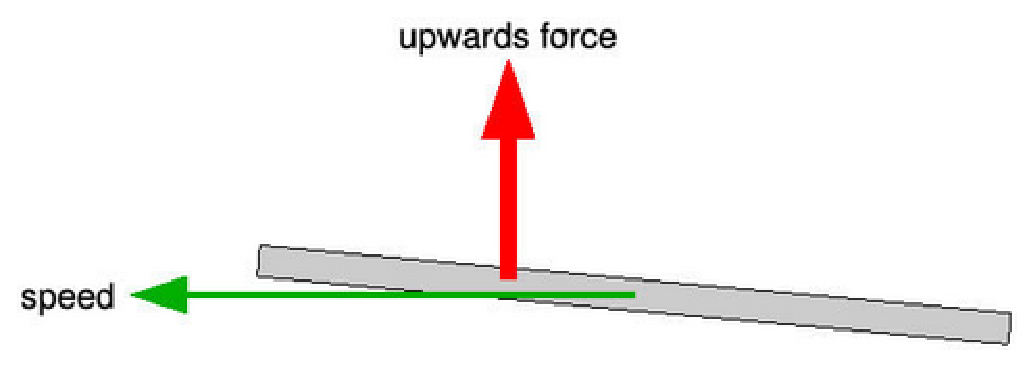
\includegraphics[width=0.5\textwidth]{img/tut_31}
\end{center}

\begin{itemize}
	\item When you pull the yoke, the airplane's nose rises up. Hence the wings 
  travel through the air at a steeper angle. Hence the lift force on the 
  wings is stronger. Hence the plane rises in the air.
  \item When you push the yoke, the airplane's nose dives. Hence the wings 
  travel through the air with less angle. Hence the lift force on the wings 
  decreases. Hence the plane descends.
\end{itemize}

What matters is the angle the wings travel through the air. This is the
angle of attach.

I wrote above that when the wings travel through the air with no angle of 
attack, they don't produce lift. This is false. It would be true if the wings 
were a flat plate like the cardboard. But they aren't. The wings are a
slightly curved airfoil. This makes them create lift even when traveling 
through the air at no angle of attach. Actually, even with a little negative 
angle of attack they still create a lift force. At high speed the airplane 
flies with the wings slightly angled towards the ground! 


\begin{center}
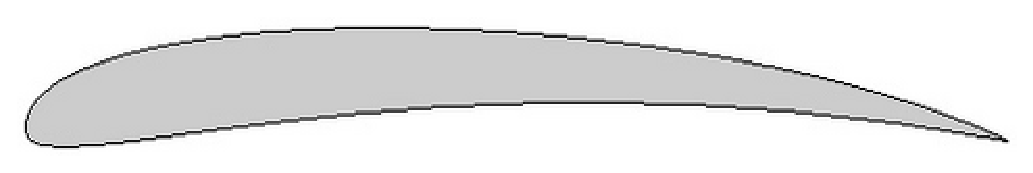
\includegraphics[width=0.5\textwidth]{img/tut_32}
\end{center}
    
The angle at which the wings travel through the air matters. Something
else matters too: the speed. Take the cardboard again in your hand.
Hold it with a given slight angle and don't change that angle. Move it at 
different speeds through the air. The faster you move the cardboard, the more 
upward force it experiences.
\begin{itemize}
	\item When you increase the engine power, the plane increases speed, the 
  lift force on the wings increases and the plane gains altitude.
	\item When you decrease the engine power, the plane decreases speed, the 
  lift force on the wings decreases and the plane loses altitude.
\end{itemize}

To make things a little more complicated: when rising in the air, the
airplane tends to lose speed. When descending, it tends to gain speed.

That's all a matter of compromises. If you want to fly at a constant
altitude and at a given speed, you will have to tune both the engine
power and the yoke/elevator (or better: the trim (see below)), till you
get what you want. If you want to descend yet keep the same speed, you
have to push the yoke a little and decrease the engine power. And so
on. You constantly have to act both on the engine power and on the
yoke. (During a normal flight one doesn't make things that complicated.
Simply tune in a comfortable engine power level then forget about it
and rely on the yoke and trim for the altitude.)

A very interesting exercise you can perform with the simulator is to
fly straight with full engine power. Get maximum speed while keeping in
horizontal flight. Then decrease the engine power to minimum. Pull steadily 
on the yoke to keep the plane at constant altitude.
The plane slows down steadily, meanwhile you have pull more and more on the
yoke to stay level. Since the speed decreases the lift of the wings 
would decrease, but you compensate the loss of speed by increasing the wing 
angle of attack. This proves the plane does not necessarily travel in the
direction its nose is heading. In this experiment we make the nose rise
in order to stay at constant altitude. Once the plane is flying very slowly, 
and the nose is very high, you may hear a
siren yell. That's the stall warning (see below). The angle of attack
of the wings is too high for the airfoil to produce lift. The wings are 
now braking the airplane instead of lifting it. The plane quickly loses 
altitude. The only thing you can do to correct this is push the
yoke forwards, making the nose drop, apply full power to gain speed and 
then bring the yoke carefully back to level flight.

Question: is it better to control the airplane's speed and altitude
with the yoke or with the throttle? Answer: it depends on what exactly
you intent to do and on the situation you are in. In normal flight, as
said above, you tend to set a comfortable engine power level, forget
about it and rely on the yoke and trim. During take off and landing the
procedures are quite strict about the use of yoke and throttle. You do
the opposite: control the speed with the yoke and trim, control the
altitude and descent speed with the engine throttle. That will be
discussed in sections below.

\subsection{The flaps} \index{flaps}
\label{sec:Flaps}
    
The flaps are situated at the rear of the wings, aside the plane's body:


\begin{center}
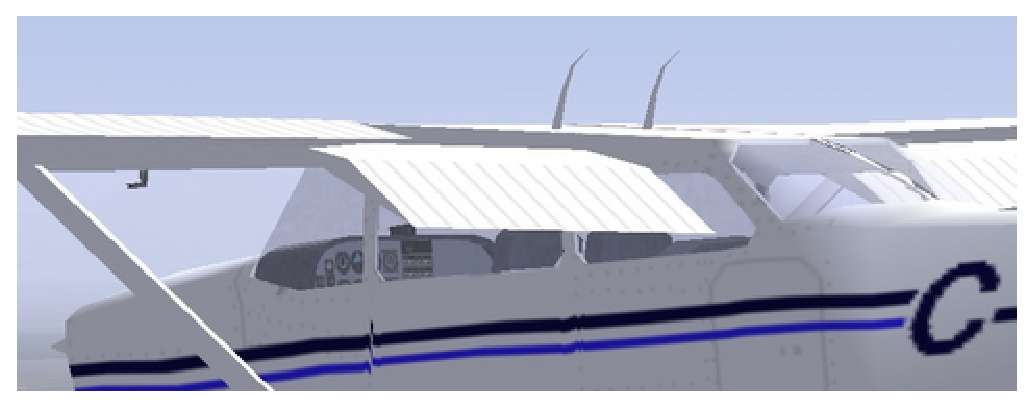
\includegraphics[width=0.5\textwidth]{img/tut_33}
\end{center}

Deploy the flaps and pull them back in by using the 
\index{flaps!control lever}flaps control lever:


\begin{center}
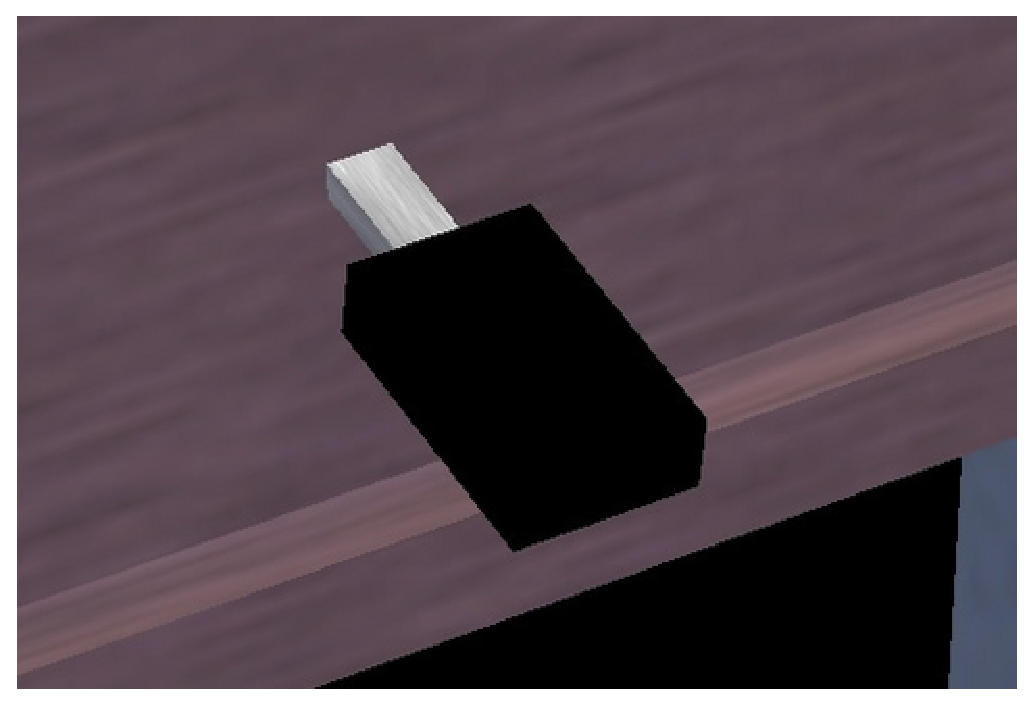
\includegraphics[width=0.25\textwidth]{img/tut_34}
\end{center}

You can either click on it with the mouse or use the \key{[} and
\key{]} keys. Key \key{[} to retract the flaps one step, \key{]} to
deploy them one step at a time. Type \key{v} to view the plane from the outside
and try out \key{[} and \key{]}. (On the schematic instrument panel the
flaps lever is located at the lower right.)

There are four \index{flaps!steps}flaps steps:
\begin{itemize}
	\item No flaps. For normal flight.
	\item One flaps step. For take off, when you want to gain altitude while flying slowly. Or during runway approach, while flying at constant altitude.
	\item Two flaps steps. To brake the plane, in order to lose altitude quickly, for example when you dive towards the runway to land.
	\item Three flaps steps. To lose altitude even more quickly. 
\end{itemize}
    
The flaps are somewhat delicate. Do not deploy the first step of flaps above 
110 knots. Do not deploy the second or third stage of flaps above 85 knots.

The flaps brake the plane at high speed. This is one more reason not to
forget to pull the flaps back in once you fly above 85 or 110 knots.

My favorite way to know the flaps position is to type
\key{Shift}-\key{right arrow}. Then quickly \key{Shift}-\key{up
arrow} to get back to front view. Another method I use is to make
sure the flaps are fully retracted by quickly typing [ several
times. Then type ] the exact amount of times needed.

Flaps increase wing lift by altering the shape of the airfoil. The wing lifts
more at a given speed with the first stage of flaps set. Hence you will get in 
the air a little sooner during take off. It also has the effect to make the 
plane fly with the nose a little more downward. This is handy: it allows to 
keep an eye on the runway while rising in the air. It also allows a better 
view on the runway during landing.

The flaps also incrase drag on the aircraft. The second and third stage of
flaps produce much more drag than lift, so they are used to brake the 
plane. This is particularly useful when landing, because the airplane glides 
very well. If you cut down the engine power completely, the plane will descend, yet
but too slowly. You need to deploy two or three flaps steps in order to
brake and really descend towards the ground.

The fact that the flaps brake during landing makes you need more engine
power during the landing. This can seem odd. Why not simply throttle
the engine down to minimum and use less flaps steps? The answer is that it is
better to have a strongly braking plane and lots of engine power,
as the plane reacts faster to your commands. Should the
engine fail, then just retract flaps as needed and your \ldots

Trying to take off with two or three flaps is a bad idea. This can
sound fun, but beware: suppose you deployed one flaps to take off. Yet
you forgot to pull the flaps back in. Later on you encounter a
emergency situation and you need to gain altitude very fast. You deploy
one flaps step. Actually you add one flaps step to the flaps step
already out. So now you have two flaps steps. Hence the flaps are
braking and you fail to gain altitude\ldots Whenever you feel the plane
is behaving really odd and seems unable to rise in the air, or even
keeps falling whatever your efforts and the engine power, think maybe
you deployed more than one flaps steps.

Redundancy\ldots What can you do if the flaps don't deploy and you
really need to brake? Answer: slowly push the rudder pedals on one
side. This will make the plane present its flank to the air stream and
brake. Compensate the turning by using the ailerons (yoke). This is not
a very comfortable way to brake and you should train it before using it
close to the ground. (I tried to use both the full flaps, the rudder to
an extreme and the throttle to minimum. You really loose altitude very
quickly\ldots)
    
    \subsection{The stall}\index{stall}
    \label{sec:Stall}
    
    
A \weblong{http://en.wikipedia.org/wiki/Stall}{stall} is an emergency
situation, at whatever altitude. It means the plane is flying too
slowly hence the wings travel through the air at too strong an angle.
The wings suddenly start braking the plane instead of lifting it. It is
especially dangerous when close above the ground. It is dangerous even
at high altitude because you lose part of your control over the plane.

During a normal flight, a stall should never occur. As a pilot you have
to constantly keep the plane well above stall speed. Once the stall
siren yells, it means things already have gone very bad.

Some little airplane like the Piper Cub are designed to land using a
near stall. Planes like the Cessna 172 are designed to make stalls less
likely to occur and less deadly when they occur. That's for example one
reason why the wing extremities are square. The Cessna is still
controllable during a stall and a simple stall and fast descent to the
ground should not kill the passengers. (Wind turbulences or a strong
bank can make things go worse\ldots)

A stall can make some airplanes go into a deadly
\weblong{http://en.wikipedia.org/wiki/Spin_(flight)}{spin}\index{spin}.
Fly for example the F-16 Falcon to some altitude, throttle the engine
down to minimum and pull steadily on the yoke to keep the same altitude
while decelerating\ldots One problem with the legendary WWII fighter
plane Spitfire was during too tight turns the inside wing would
suddenly stall completely but not the outside wing.

What can you do during a stall? The procedure can be very different on
different planes. You should not trust this tutorial, especially not
for such a serious matter. Anyway:
\begin{itemize}
	\item On little planes like the Cessna 172p or \index{stall!little planes}the Piper Cub you keep all controls on the airplane: elevator, rudder and both ailerons. Keep in mind the ailerons are on the wings and those wings are stalling. Think of using the rudder to turn. If you are very close to the ground, simply let the plane fall on the ground and keep it on the ground. Just try to make the best possible fall. If you are high in the air, push the yoke to dive the nose and gain speed. Think of retracting the flaps at one step. If possible, immediately add as much engine power as you can. Till you are out of danger.

	\item On the F-16, \index{stall!greater aircrafts}the ailerons loose all control during a stall. Actually that's the first sign of a stall: the ailerons act no more and the plane banks loosily. You only keep control with the rudder and the elevator. If the stall just begins, dive the nose and increase engine power. If the stall degenerated in a spin, engine power and dive won't solve the problem. Only the rudder will help to slow the spin down. Push the rudder to the other extreme of the spin direction. Push the yoke to help. Decrease engine power to minimum to get out of the spin more easily. Once the spin is slow enough, a dive and engine power will help. (If you put full engine power during the spin, you will loose less altitude I believe, but the spin's end will be difficult to control. React quickly to center the rudder again once the spin nearly stops, otherwise you will immediately go spinning in the other direction.) At low altitude you probably won't have the time to do all this. Note a spin with the plane belly up can happen too.


\end{itemize}

Stall-elegant airplanes like the Piper J3 Cub and the Cessna 172 tend
to have roughly rectangular wings. While stall-ugly airplanes like the
F-16 Falcon and the Cessna Citation II tend to have trapezoidal wings.
The advantage of the trapezoidal wings is they have a better
aerodynamic yield. They allow to fly more distance with a same quantity
of fuel. The ends of the rectangular wings engender strong turbulences.
Those turbulences brake the plane but also they keep the air flowing
correctly once the plane stalls...

When you learn to fly a virtual plane, making it stall is a very good exercise:

\begin{itemize}
	\item Fly at constant altitude with no engine power, till the stall begins. Then try to control the plane while it stalls and descends to the ground. Keep the yoke pulled to the maximum. Keep the plane in a steady attitude, the wings parallel with the horizon. Try to change direction. Experiment with the flaps. Note one flaps step decreases the stall speed. Two or more flaps steps don't change the speed much. Then end the stall by pushing the yoke and restoring engine power.
  \item Raise the nose in the air and bring the plane to a halt like a stone thrown upwards. Then try to get the plane back to normal flight.
\end{itemize}

Try to perform the exercices above with different airplanes. You will
notice how elegant the Cessna 172p behaves. First time I tried a stall
with the virtual Cessna Citation II, I was at 1,000 feet altitude,
which is supposed to be safe. The plane suddenly fell from the sky like
a tumbling stone. I was not able to stabilize the plane and it crashed.
I was really frightened by that airplane. On second attempt I managed
to stabilize before the plane hit the ground. Anyway, from now on I
won't fly a Cessna 172p and a Cessna Citation II with the same mood.

If you fly an unknown virtual airplane and wish to know the landing
speed, a rule of thumb is you find out the stall speed by
experimenting. Then you multiply that speed by a factor of 1.2 or more.
(A friend who is Aerospace Engineer told me 1.2.) The stall speed of
the Cessna 172p is 40 knots yet its imposed landing speed is 70 knots
(minimum 65 knots). That makes a factor of 1.75\ldots I made an
experiment landing the virtual Cessna 172p at 50 knots. It virtually
falls to the ground, at close to -1000 feet/minutes vertical speed.
This seems very hard for the landing gear. Next, while approaching at
50 knots with the Cessna 172p, the runway and most of the ground are
completely hidden. This obviously tells a higher speed is mandatory. I
would recommend following rules to find a correct landing speed. It
must be the lowest possible speed that satisfies all these conditions:
\begin{itemize}
	\item Be more than $1,2\times$ \hspace{-2pt}the stall speed.
	\item Be high enough to allow a vertical speed of no more than -500 feet/minute (all or most flaps steps deployed).
	\item On most modern planes, the landing speed must be high enough to allow you to see the runway while approaching at low speed and constant altitude.
\end{itemize}
On big jet airliners the flaps make a lot of difference. Bear that in
mind when you try to find the stall speed. Make the experiment with the
flaps deployed, as they will be deployed during the landing.

The load of the airplane also changes the stall speed a lot, and
therefore the landing speed. You land a fully loaded airplane at a
higher speed than an empty one.

(Once you get used to landing different airplanes, you get a feeling for the landing speed of an unknown airplane. You just feel the airplane "wants" to land at that speed. I suppose this is because the airplane was designed to land at that speed.)

\excl{In a real airplane the sounds and vibrations tell a lot about the state of the airplane. When all vibrations stop, this means you are going to stall. Then push the yoke to get speed.}

   
    \subsection{The trim}\index{trim}
    \label{sec:Trim}
    
    The trim is that dark big vertical wheel with gray dots located at the middle below the instrument panel:
    
    

\begin{center}
\includegraphics[width=0.25\textwidth]{img/tut_35}
\end{center}
    
  On \fg, the keys \key{Home} and \key{End} are used for the trim. The key \key{Home} rolls the wheel upwards while the key \key{End} rolls the wheel downwards. You can also click on the upper or lower half of the trim wheel (\key{Ctrl}-\key{c} for a yellow highlight). Possibly look at the plane from the outside (\key{v} or \key{V} and \key{x}) and move the trim while looking at the elevator.

In first approximation, the trim does the same as the yoke: it acts on
the elevator. Turning the trim wheel downwards is the same as pulling
on the yoke. Yet there is a key difference between the trim and a real
yoke. If you tune the trim, it keeps that tuning. While if you pull or
push on the yoke, it goes back to neutral once you release it.

Once in flight, you would keep the mouse/yoke at a given forward (or
backward) position. That position is optimal to keep the plane at a
roughly steady altitude. In a real airplane, this means you would
constantly keep pushing (or pulling) on the yoke. That would be quite
uncomfortable. This is where the trim falls in. You tune the trim to
impose a default elevator angle. Then you no longer have to push or
pull the yoke constantly. In other words: make a global rough tuning
with the trim and occasional fast tunings with the yoke/mouse.

The trim is an important control. I tend to forget it, for two reasons.
First is the mouse makes the trim virtually useless. This is quite
unnatural of course. People with a force-feedback joystick/yoke will
feel the need for the trim, as well as people flying real airplanes.
Second is the trim didn't operate on the particular version of
FlightGear I was using until recently\ldots

During take off the trim must be neutral. You have to check the trim is
centered before every take off. Also if you abort a landing and start
rising back to altitude, put the trim to neutral. Otherwise the plane
may buck.

During landing, while flying at a constant speed of 70 knots and a
constant altitude of 500 feet, the same applies as for a steady flight:
try to get the yoke/mouse/elevator towards neutral position by tuning
the trim. On the Cessna 172p this means trim on neutral (except when
the plane is loaded). On the Cherokee Warrior II this means the trim a
little ``pulled''.

During the final dive, some people seem to let the trim as it is and
use the yoke, others make the dive using the trim and don't use the
yoke/elevator. I don't know which is best. I use the yoke.

To know the trim position, use the HUD (\key{h}, \key{H} and \key{I})
or the I-shaped indicator on the schematic instrument panel (\key{P}).

The trim movement is very slow. Be patient.

Lots of modern airplanes have a remote control for the trim: a little
switch on the yoke, that you can manipulate easily with your fingers.
So you don't have to duck to roll the big wheel.

    
    \subsection{What direction am I flying?}
    \label{sec:Kierunek}
    
    Four basic methods exist to know what direction you are flying:
    
\begin{itemize}
	\item Look through the windows. Try to learn and recognize all sorts of ground features, like hills, bridges, cities, forests\ldots The Sun and the Moon are essential features, but clouds can cover them and they move through the sky. Looking through the windows can be quite hectic on a flight simulator. You only have a narrow view on the virtual outside world. Using two more displays, placed left and right of the main one, will help. Yet this is expensive and not mandatory. Several ways exist to allow you to pan your virtual head inside the airplane: 
	  \begin{itemize}
    	\item [$\rightarrow$]Use \key{Shift} and the four \key{arrow keys} to look frontwards, backwards, leftwards and rightwards.
    	\item [$\rightarrow$]Use \key{Shift} and the keypad keys to look in the four directions mentioned above and in four diagonal directions in-between
    	\item [$\rightarrow$]Put the mouse in pan mode (right button,  $\leftrightarrow$cursor look). This allows you to look in just every direction, including towards the sky and towards the ground. This method is great while the autopilot is on. It is a little dangerous otherwise, because the plane will bank or fall while you're looking all around. Click the left mouse button to quickly get back to the default forwards vision. Hint: if you click the left mouse button to center the vision back, by the time you click the right mouse button to go out of mouse look mode you will already have panned a few degrees away from the forward view. This is not a serious problem, except for the fact it prevents the instrument panel to appear when typing \key{P}. A solution is to lift the mouse before you click the left button. Then click the right button. Then let the mouse back down. (While the autopilot is on and you are looking all around, use the \key{x}, \key{X} and \key{Ctrl}-\key{x} keys to zoom in and out. Use the \key{z}, \key{Z} and \key{Ctrl}-\key{z} keys to dissolve the mist outside.) %
    \end{itemize}
  \item The compass (picture below). This is the indicator located above the instrument panel. The compass is a very simple and classical, yet not perfectly reliable instrument. When flying over some places, magnetic perturbations on the ground can make the compass tell nonsense. Also, the compass never shows the real direction of the North, East or South. Rather it shows a direction a few degrees aside from the real direction (depending on the country you are in). Close to the poles the error of the compass becomes really strong.  


\begin{center}
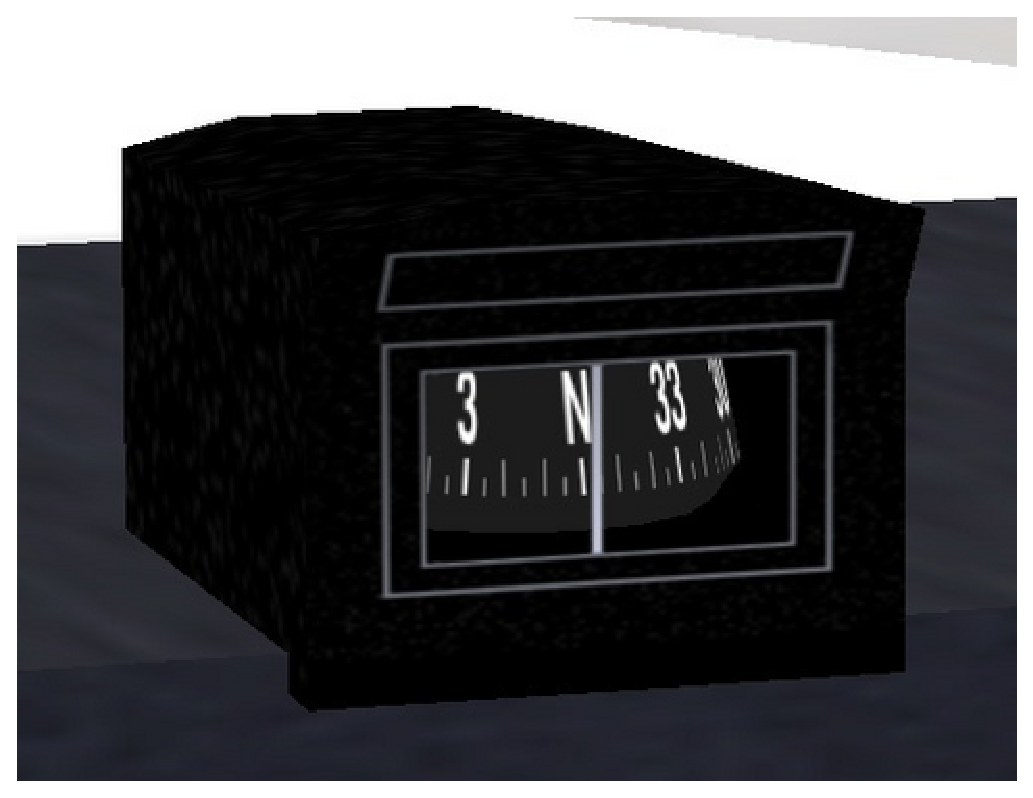
\includegraphics[width=0.25\textwidth]{img/tut_36}
\end{center}


  \item The directional gyro (picture below) or ``heading indicator''. The gyro is started before take off and keeps its initial heading for hours. It simply tells you how many degrees you turned to the left or to the right. You are supposed to tune in the right direction of the North Pole before you take off, using the knob at the bottom left of the instrument (normal mouse pointer mode, click left or right half of the knob, middle mouse button to move faster, \key{Ctrl}-\key{c} to highlight halves). (The red knob, bottom right, is used to tell the autopilot what direction you wish to fly (\textcolor{red}{\button{HDG}} = ``heading'').


\begin{center}
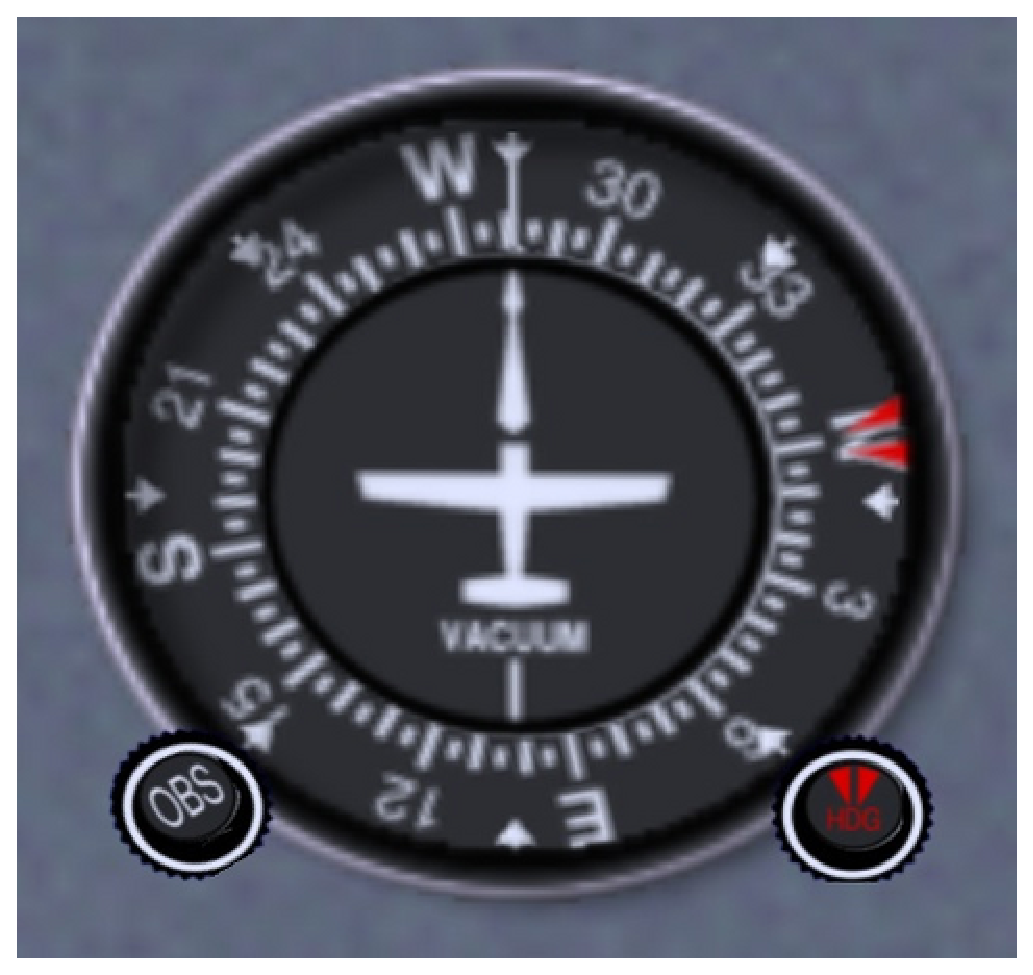
\includegraphics[width=0.25\textwidth]{img/tut_37}
\end{center}

  \item The clock. If you make steady turns, at the angle proposed by the turn indicator, a 180� turn takes 60 seconds whatever the flight speed (yet it is 50 seconds on FlightGear\ldots).

\end{itemize}    

  \excl{During a real flight in a real airplane, you are supposed to cross-check all direction indicators once in a while.}

Memorize the directions: North is 0$\textdegree$, East is
90$\textdegree$, South is 180$\textdegree$ and West is
270$\textdegree$.

  \section{Let's Fly}  
    \subsection{A realistic take off}
    \label{sec:Start}
    
By now I assume you are able to keep the airplane on the runway while
taking off (rudder) and you're able to fly straight, descend
peacefully, gain altitude steadily, make gentle turns (yoke)\ldots No
need you perform this all perfectly. Yet a basic and approximate
control of the airplane has been acquired.

Rules during \weblong{http://en.wikipedia.org/wiki/Take_off}{take off}: 
\begin{itemize}
	\item You are not allowed to keep the front wheel on the ground above 40 knots. It would shimmy.
	\item When close to the ground (I don't know the exact limit) you have to keep the two rear wheels at the same height above the runway. The reason is any moment you will or may touch the ground. You need to touch with both two rear wheels together. That means you need to keep the wings level with the horizon. Hence you cannot make use of the yoke/mouse/ailerons to turn. Instead you use the rudder pedals to turn. (Since you fly around 70 knots, this yields not too much sideways force problems.) The yoke/mouse/ailerons are used to keep the wings level with the horizon.
  \item You are not allowed to fly lower than 500 feet above the ground. The sole exception is in the axis of the runway, during take off and during landing. (While flying over cities you are not allowed to fly lower than 1,000 feet above the ground.)
  \item When lower than 500 feet above the ground, you are not allowed to fly \emph{slower} than 70 knots speed. That's because a blow of wind from the rear can occur any moment. You need to fly fast enough so that such wind blows won't make the plane stall and fall to the ground.
  \item When lower than 500 feet (above the ground), you are not allowed to fly \emph{much faster} than 70 knots. You wouldn't be able to make maneuvers quick enough. You would be more destructive if you hit something. Besides, 70 knots is a nearly optimal speed to gain altitude and your sole acceptable purpose while lower than 500 feet is to gain altitude\ldots
  \item While taking off, you must stay aligned with the runway. Indeed that's the sole place you are allowed to fly below 500 feet. (If you take off from a long runway like KSFO, this also allows to land back safely and quickly should an emergency occur. (Above a short runway, you cannot simply dive and get back on the runway, because it is too short. You need to turn and circuit to make a regular landing. For this you need to have enough engine power or to be at least at 500 feet above the ground. Otherwise, quickly find a place where you can make an emergency landing.)) 

\end{itemize}

So, you need to take off and rise in the air at a steady speed of around 75 knots.

Problem: since the front wheel is slightly lifted and the flaps are one
step deployed, the plane will rise from the ground already at 55 knots.
That's well below the desired flight speed of 75 knots. What to do
then? Answer: as soon the two rear wheels lift from the ground, push
the yoke forwards a little. Keep the plane close above the ground. (The
aim of this is: should a wind blow from the rear occur, the plane will
fall from only a few feet hight.) Keep it close above the ground while
accelerating, till a speed of about 70 knots is reached. Then switch to
the opposite mode: now you must pull on the yoke to prevent the plane
from going above 75 knots. Force the plane to rise in the air, so it
doesn't gain speed. Keep in control. If the speed goes below 75 knots,
push a little on the yoke. If it rises above 75 knots, pull a little on
the yoke. Till you reach 500 feet above the ground.

This is the procedure I use to take off. I assume you just started \fg; the airplane is at the start of the runway and the engine is turning at minimum power:
\begin{enumerate}
	\item Get a HUD ( \key{h}, \key{H}, \key{i} and \key{I}) or the schematic instrument panel with the I indicator (2D panel aircraft from start or key \key{P}).
	\item Deploy one step of flaps (\key{]}).
	\item Get in mouse yoke mode ($+$ pointer shape) by clicking on the right mouse button.
  \item Pull the yoke/mouse/elevator to 1/2 the total way: 


\begin{center}
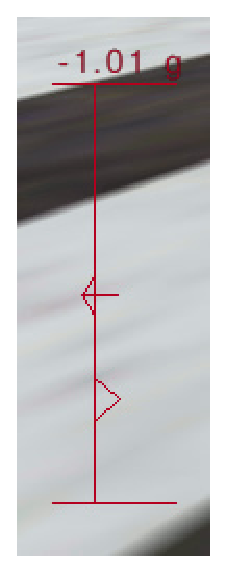
\includegraphics[width=0.25\textwidth]{img/tut_38}
\end{center}

  \item Ensure the yoke/mouse/ailerons is centered: 


\begin{center}
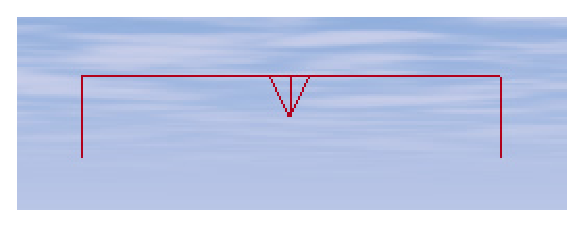
\includegraphics[width=0.25\textwidth]{img/tut_39}
\end{center}

  \item Push the left mouse button down and keep it down, so the mouse gets in rudder control mode. (If you don't want to use the mouse to control the rudder, use the keypad \key{0} and \key{Enter} keys.) (Before you push the left mouse button, ensure the yoke/elevator is pulled 1/2 like asked above and the yoke/ailerons is centered.)
  \item Keep the \key{Page Up} key down till the engine roars at its maximum power.
  \item The airplane is now accelerating. Move the rudder/mouse to the left and to the right to keep aligned with the runway (the left button is pressed). You need to keep in the middle of the runway but this does not need to be very precise. More important is your path is parallel with the runway middle line and stable. 
  
  \item Because the yoke/elevator is pulled $1\over2$ in, around 40 knots the nose will rise up. Immediately release the left mouse button, to get back in yoke control mode. Immediately push the yoke/mouse a little bit, to keep the engine cover below the horizon. You just need to let the front wheel rise a little bit above the runway. Let the rudder keep its angle (probably slightly turned to the right; two keypad \key{Enter} hits from the center position). From now on keep the left mouse button released, to stay in yoke control mode. Use the keypad \key{0} and \key{Enter} keys to control the rudder. (You can also make short presses on the left mouse button to make little rudder adjustments. I prefer using the keys.)
  
  \item The airplane soon leaves the ground. The two rear wheels no longer touch the runway. Push the mouse a little, to prevent the airplane from rising in the air. Keep it flying close above the runway and aligned with it. (Do not try to stick really close to the ground. This would be dangerous. Let the plane rise a little bit. Just do not favor the rising.)
  \item Use the yoke/ailerons/mouse to keep the wings level with the horizon. Use the rudder/keypad \key{0} and \key{Enter} to turn (needs training). Optimal rudder position seems to be slightly right from neutral; two keypad \key{Enter} hits.
  \item Once the airspeed reaches 70 knots, pull on the yoke/mouse a little bit. Now the airplane firmly rises in the air. If the speed gets below 75 knots, push the yoke to force the airplane to rise slower and gain airspeed. If the speed rises above 75, pull the yoke to rise faster and decrease the airspeed. There is no need to be very precise. Try to keep a stable speed. Just avoid to go below 70 knots and above 80 knots.
  \item Don't keep your eyes too much on the speed indicator while you are rising above the runway. Rather look at the horizon and at the engine cover. The top of the engine cover should roughly match with the horizon line:


\begin{center}
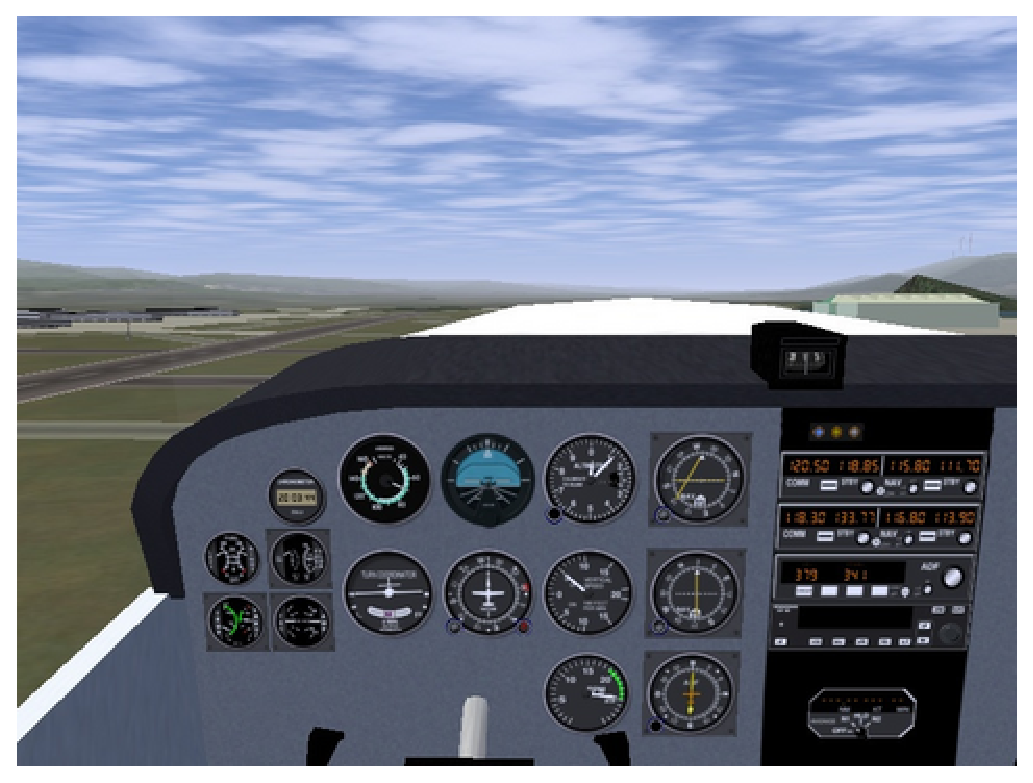
\includegraphics[width=0.5\textwidth]{img/tut_40}
\end{center}
  
  \item If you want to check the position of the runway but you can't see it because it is hidden by the engine cover, push the yoke/mouse a short while to make the nose dive a little bit for a second. This only works for long runways. Another trick is to look for a building, a hill or something far in front of the runway, on the horizon. Keep aiming at that object while rising in the air. Keep the engine cover a little below the horizon line, so the object you aim at stays visible.

  \item Once you reach 500 feet, retract the flaps (\key{[}) and push the yoke a little. Center the rudder (slowly, one step at a time). You are now allowed to gain speed or go on climbing (your choice, or the control tower's). Decrease the engine power a little so the RPM needle gets in the green zone (\key{Page Down}). Turn calmly towards your intended flight direction. Use your time to optimize the mixture. You're in flight.  
\end{enumerate}    
    
500 feet above the ground is the minimum flight altitude above open
land. Above a city the minimum altitude is 1,000 feet.

If you take off from KSFO heading to the West, you have city areas in
front of you and left of you. So, once you reach 500 feet above the
ground, best turn to the right.

Don't forget to center the rudder. If the rudder is pushed to one side,
this will brake the plane. It makes the plane move sideways through the
air, with its flank aerobraking.

Don't forget to retract the flaps.
    
    \excl{During a real take off you must keep in touch with the control tower. You also have to constantly look in all directions to check no other airplane is coming in your direction. }
    
An aviation classic is the
\weblong{http://en.wikipedia.org/wiki/Ground_effect}{ground
effect}\index{ground effect}. It's the fact a wing lifts better when
close above to the ground. That too makes the wheels leave the ground
at quite a low speed, a speed at which the airplane cannot really fly.
While you are accelerating a few feet above the runway, you are in
ground effect. If you know about it, ground effect is an advantage
because it makes flying close above the ground more secure. The
airplane behaves a tiny little bit like a hovercraft. If you are not
aware of the ground effect, it can cause problems. For example it can
make you think the airplane has enough speed to rise in the air, while
it has not.


    
    \excl{During a real take off, if the engine halts below 500 feet, you are not allowed to turn and try to glide and land back on the runway. You only have enough height to try to turn and land back if you are above 500 feet when the engine halts. }
    
    \excl{Before a real take off you have to go through check-lists. A checklists makes you verify, tune and tighten a list of items. You have to follow a long checklist before you enter the runway and a short checklist before you accelerate to take off.}
    
This is the checklist I follow when I take of the virtual Cessna 172p
on \fg. It is very short compared to a real checklist. Anyway I know I
can go into (moderate) trouble if I don't follow it. I had to build up
the discipline to follow it carefully each time:

\begin{itemize}
	\item Check the wind direction
	\item Deploy one step of flaps.
	\item Click the right mouse button and ensure the mouse is in yoke mode ($+$).
	\item Put on a HUD (\key{h}, \key{H}, \key{i}, \key{I}) or the schematic instrument panel  (\key{P}) in order to know the controls positions.
	\item Pull the yoke/mouse to $1\over2$ the pull path.
	\item Check the yoke/ailerons are centered.
	\item Keep the left mouse button down and check the rudder is centered or slightly to the right.
	\item Keep the  \key{Page Up} button down to start accelerating, till the engine RPM is maximum.
\end{itemize}

    
    \subsection{Landing}\index{landing}
    \label{sec:Ladowanie}
  
When I was a boy, I had a simple yet fairly good flight simulator on my
\weblong{http://en.wikipedia.org/wiki/ZX_Spectrum}{Sinclair ZX
Spectrum} home computer. I could do everything with it, except landing.
I always crashed the plane, or reached the end of the runway before
stopping. One day a real pilot saw me trying to land. He had never seen
a flight simulator, but he had no problem to recognize each flight
instrument and ground feature on the screen. He told me what to do.
Decrease engine power, increase engine power, push the nose down, pull
the nose up, turn a little left, turn a little right, get the flaps
out\ldots We made a perfect landing on the second attempt.
  
  Just like for take off, \weblong{http://en.wikipedia.org/wiki/Landing}{landing} is partly a procedure, partly rules you have to stick to. You have to adapt constantly.

  Same basic rules apply as for take off, yet in reverse order:
\begin{itemize}
	\item Stay at 70 knots once below 500 feet. Descend towards the \weblong{http://en.wikipedia.org/wiki/Runway}{runway} while keeping at 70 knots. 
	\item After the final rounding (see below), stay close above the runway while decreasing speed from the 70 knots flight speed down to the roughly 55 knots landing speed.
	\item Touch the runway with the two main wheels. Keep the front wheel from the ground till the speed is below 40 knots.
\end{itemize}

(If you know what you are doing you are allowed to use a speed a little below 70 knots: 65 knots.)

Following rules are essential during the whole procedure of landing:
\begin{itemize}
	\item Tune the speed using the yoke/mouse/elevator: push the yoke if you are flying below 70 knots, pull the yoke if you are flying above 70 knots. No matter this makes you gain or lose altitude (except when this causes a danger of course).
  \item Tune the altitude using the engine throttle. Add power if you are too low, retract power if you are too high.
  \item Once approaching the ground, use the yoke/ailerons to keep the wings level with the horizon. Turn using the rudder.
  \item Don't shut the engine down. Only shut the engine down when the airplane is completely halted on the ground. There are two reasons for this:
\begin{itemize}
	\item [$\rightarrow$] Any moment you may need full engine power to rise back in the air.
  \item [$\rightarrow$] Engine thrust enables you to make more precise landings. For example if you land on a very short runway, you need that precision.
\end{itemize}
\end{itemize}

The reason why the yoke/elevator is used to tune the speed is this
method allows for fast reactions and fine tuning. It is more important
to tune the speed closely than the altitude.

If you are both a little too high and a little too slow, simply push
the yoke a little and both problems will be solved together. No need to
use the throttle. Use your mind...

You have to get aligned with the runway. That means your flight
direction has to match the middle line of the runway (drawing (a)
below). In order to arrive at this, don't aim at the start of the
runway (b). Rather aim at a fictitious point well ahead of the runway
(c). And begin to turn gently towards the runway well before you reach
that fictitious point (d). Note the turns and bankings you make for
these flight corrections are often very soft. You wouldn't even notice
them on the turn coordinator. This is one example where you better rely
on the outside horizon line than on the inside flight instruments.


\begin{center}
\includegraphics[width=1.0\textwidth]{img/tut_41}
\end{center}

Try to get aligned with the runway as soon as possible. Constantly
apply the alignment procedure. The closer you come to the runway, the
better the alignment should become.

My favorite landing procedure for the Cessna 172p is roughly this one:
\begin{enumerate}
	\item Far from the runway, yet already heading towards it, start decreasing the speed and let the plane descend towards 500 feet. 
	\item Check the rudder is neutral. Otherwise the plane will be braking and more engine power is needed. (Type keypad keys \key{0} and \key{Enter} to center the rudder if needed.) If you make corrections using the rudder, keep in mind you may need a little more engine power.
	\item Once the speed is below 100 knots, deploy one flaps step  (\key{]}). 
	\item Once an altitude of 500 feet is reached, keep that altitude. Once a flight speed of 70 knots is reached, keep that speed. (If in doubt, keep above 500 feet.) The exact altitude doesn't matter much provided it is stable. But stick to 70 knots.  
	\item Be firm with the flight speed. Keep a tight and quick control on the yoke/mouse to keep 70 knots. If the speed is lower than 70 knots, push the yoke to gain speed (no matter you lose altitude). If you are above 70 knots, pull the yoke to lose speed (again, no matter this makes you gain a little altitude). Don't panic if the speed rises to 75 knots or decreases to 65 knots. But keep in mind you can really get in trouble if you approach a short runway at 80 knots. I manage to keep the speed between say 68 and 72 knots.  
	\item Tune the trim to get the average position of the yoke/elevator centered. This is not mandatory on the simulator, yet that way you better mimic piloting a real airplane. On the Cessna 172p (with no load) this means trim on neutral.
	\item Be firm with the flight speed. Keep a tight and quick control on the yoke/mouse to keep 70 knots. If the speed is lower than 70 knots, push the yoke to gain speed (no matter you lose altitude). If you are above 70 knots, pull the yoke to lose speed (again, no matter this makes you gain a little altitude). Don't panic if the speed rises to 75 knots or decreases to 65 knots. But keep in mind you can really get in trouble if you approach a short runway at 80 knots. I manage to keep the speed between say 68 and 72 knots.
	\item Fly at constant speed and steady altitude towards the runway. 70 and 500. Keep trying to align with the runway. You will \textbf{never} be perfectly aligned. You have to go on aligning till the airplane halts on the runway.
	\item Now you are at a low flight speed of 70 knots, no more use the ailerons/yoke to turn. Instead use the ailerons to keep the wings horizontal. Turn using the rudder (Keypad keys \key{0} and \key{Enter}). The rudder can seem an odd device for this purpose yet you will get used to it. Move the rudder only a few key hits to the right or to the left. Be patient. Make one key hit at a time and allow the airplane to stabilize before you possibly make another key hit. (When I started making landings, I found the rudder to be hectic and I prefered to use the ailerons to turn. As experience build up, I finally found out that turning with the rudder allowed for more precise and comfortable adjustments.)
	\item The airplane may oscillate a little. Don't bother. Just keep in control using the yoke.
	\item You're flying at constant altitude and 70 knots speed. Once the beginning of the runway passes under the engine cover, it's time to take things up seriously. This is shown in the picture below. (Whatever altitude you are flying, once the engine cover begins to eat the runway, you are at a correct angle towards the runway start.) 


\begin{center}
\includegraphics[width=0.5\textwidth]{img/tut_42}
\end{center}

	\item Type \key{]} two times, to deploy the full three flaps steps.
	\item Immediately push the yoke forwards, to make the airplane plunge to the ground. Indeed, the full flaps deployed make the plane brake. You plunge towards the runway to land, of course, but also to keep the speed at 70 knots. 
	\item Decrease the engine power. $1\over4$ the maximum is often fine. The Cessna 172p needs even less. I tend to decrease the engine power throughout the dive, to end with almost no power. The possibility to add engine power is necessary for your safety and for the precision of the landing, but also the possibility to decrease the engine power. So I try to make my dives a way that I keep the engine at some decent power level throughout the dive. If a dive obviously begins with the need to decrease the power to minimum, there is a risk you touch the runway far beyond its start.
	\item Watch the speed indicator like it if was your heartbeat. Control the speed using the yoke/elevator. 
	\item The dive makes you head towards the runway. You will soon become aware that the plane is going towards a point of the runway much further than the start of the runway. There is nothing wrong with that on a long runway. Yet you should train to land on short runways. In order to correct the dive and head towards the start edge of the runway, decrease the engine power. (On the Cessna 172p this often leads to power to minimum, while on most other airplanes you keep some power tuned in.) The picture below is a snapshot from a good dive. (Note the vertical speed indicator shows $-500$ feet/minute. I never use that indicator. I solely aim at the runway edge and its 12 white strips. Anyway, -500 feet/minute is the right descend speed\ldots) 


\begin{center}
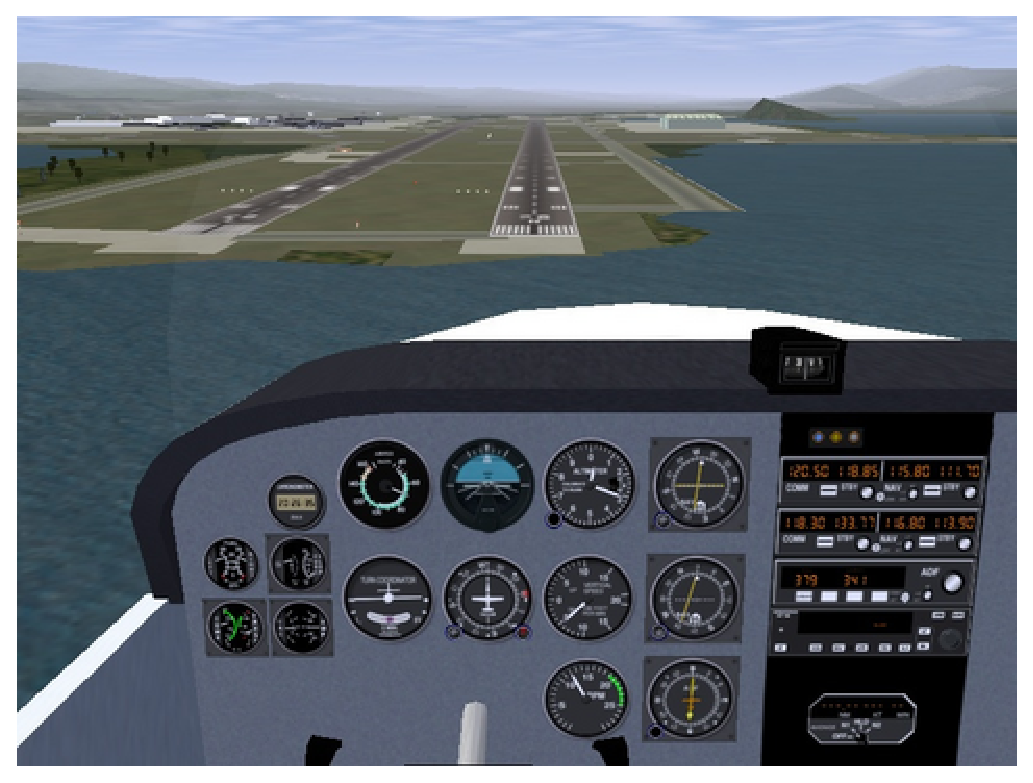
\includegraphics[width=0.5\textwidth]{img/tut_43}
\end{center}
  
  \item Closely keep the speed at 70 knots by pulling and pushing the yoke. Calmly increase and decrease the engine power in order to head the plane towards the starting line of the runway. Don't bother to aim exactly at the start of the runway. It doesn't matter if you arrive a few feet before the runway start or much further after it. Provided you arrive at 70 knots. 
  \item Keep aligning with the runway, using the rudder pedals to turn (keypad keys \key{0} and \key{Enter}). Keep the wings level with the horizon using the mouse/yoke/aile\-rons. (Use the ailerons to turn only if an emergency occurs and you need to make fast and steep turns. Then you probably need to abort the landing and get back to altitude (see below).)
  \item If you suddenly realize you will arrive really far before the beginning of the runway, possibly retract the flaps to one step (\key{[}). You can also let the engine roar to maximum power for a few seconds. If you followed the procedure you shouldn't need to do such extreme things\ldots (At any time, if you feel things are going wrong, retract the flaps to one step, throttle to full engine power, put the trim on neutral and gain back altitude (keep the speed above 70 knots). Whatever wrong happens -- you arrive aside from the runway, too far before the runway, at a wrong speed, a swarm of birds is passing, whatever -- abort the landing. Get back to altitude and retry.) 
  \item The ``\Index{rounding}'' is the most impressive part. You are like going to crash on the runway. Yet you will pull the yoke/mouse before it's too late. Don't pull on the yoke too early. Don't pull on the yoke too firmly. Once you are really close to the runway (for a beginner: once you are convinced it's too late and you are going to smash into the ground), pull the yoke gently and bring the plane in a steady flight above the runway. That's the rounding. (During the rounding, ground effect contributes to your security and ease.)
  \item It is often best to reduce the engine power to minimum during the rounding.
  \item Go on using the rudder pedals (keypad \key{0} and keypad \key{Enter}) to keep aligned with the runway. Use the yoke/ailerons to keep the wings level with the horizon (so both left and right wheels will touch the runway at the same time). 
  \item Now you're flying close above the runway (in ground effect). Throttle the engine power to minimum if it wasn't already done (this is mandatory). Deploy full flaps if they weren't already deployed completely (this is not mandatory on a long runway). (Don't shut the engine down. Just throttle to minimum power. It still can happen that you suddenly must take off again and need full power in a few seconds.)
  \item Keep the plane flying close above the runway. As the speed decreases from 70 knots down to 50 knots and below, keep pulling more and more on the yoke/mouse, steadily. Keep the plane in the air while ensuring it stays really close to the surface of the runway. Steadily lift the nose, while the plane slows down, up to quite a strong angle. Make sure the plane does not gain back altitude (don't look at the instruments, look at the outside). You really have to avoid the plane rises back in the air. Indeed it would do that at a speed below 70 knots... (You shouldn't need to pull the yoke more than $1\over2$ its maximum.) 
  \item Don't land the plane. Let it land by itself, once the speed is too low and the nose is high up in the air. The plane renounces to fly, it calmly sinks in and the two rear wheels touch the runway. If you don't hear the wheels hit the runway and the wheels nevermore leave the runway, you probably made an optimal landing. This also makes the front wheel stays above the runway while the two rear wheels touch.
  \item Once the rear wheels roll on the runway, retract the flaps. That way the wings will lift less and the plane will be more firmly on the ground. (My favorite way to land the airplane is to let the flaps down and keep pulling on the yoke while the airplane is rolling. That way I get maximum braking. I suppose this is an example of the difference between a simulator and reality. Using my way the airplane risks to get back in the air any moment and it is very sensitive to blows of wind. If I made real landings, maybe I wouldn't dare do this\ldots)
  \item When the plane is rolling, an optimal position for the yoke/elevator seems to be pulled $1\over2$ of the total way.
  \item Use the rudder pedals to keep the plane rolling in the middle of the runway and straight while the speed decreases. This most often leads me to two keypad \key{Enter} hits to the right of the center position.
  \item Once rolling at a speed below 40 knots, the nose will go down automatically. Help it by pushing the yoke/mouse calmly, back to neutral position. The front wheel now must touch the runway. Beware: check the rudder position first. If it is too much to the left or to the right, the plane will turn violently once the front wheel touches the runway. The plane may even fall aside and hit the ground with a wing tip. (The rudder slightly to the right; two keypad \key{Enter} hits, seems an optimal position.)
  \item Now the front wheel is on the ground, use the mouse to control the rudder. Keep the left mouse button down and forget the keypad keys. Maybe just check the ailerons and elevator positions are sound before you press the left mouse button. (Actually if everything went correctly and there is no crosswind, you shouldn't need to steer the plane using the rudder.) 
  \item Once the front wheel is on the ground, you are allowed to use the brakes. Your choice. Keep the \key{b} key down. Be prepared to release it should a problem occur. If you forgot to almost center the rudder, braking can go really bad.
\end{enumerate}

    Once the plane is halted or at very low speed, you can release the
    \key{b} key (if you used it) and add a little engine power to taxi
    to the parking or hangar.
 
    To shut the engine down:
\begin{itemize}
	\item Engine throttle to minimum (hold  \key{Page Down} down for a while).
	\item Pull the mixture lever to halt the engine (mouse in normal pointer mode, click on the left of the red mixture lever to pull it out).
  \item Rotate the magneto switch to OFF (a few hits on \key{\{}). 
\end{itemize}
To set the parking brakes in, type \key{B}.    
     
You must be mentally prepared to abort landing anytime. Whatever
happens: an order from the control tower, a wrong speed or landing
angle, a wrong alignment with the runway, a strong blow of wind, birds
flying over the runway\ldots retract the flaps to one, push the engine
to maximum, center the trim and get back to high altitude. Then either
you restart the landing procedure or you go for another airport. The
pride of a pilot is to make only safe landings.

Don't try to find ``the ideal distance'' to start diving to the runway.
The procedure above proposes you start diving when the white engine
cover starts eating the runway edge (provided you fly at 70 knots with
one flaps step) (the altitude doesn't matter). Best is you train to
land while starting the dive earlier and while starting to dive later.
You need to be trained to increase or decrease engine power according
to what is needed. During a real landing, depending on the airplane's
weight, the wind speed and other random things, the ``ideal'' moment to
dive is unpredictable. As experience builds up, you will better feel
the right moment.

If you want to make things simple for your first landing trainings,
make use of the fact the runway at KSFO is very long. Wait a little
more before you begin the dive: let the nose ``eat up'' the whole
length of the leading part of the runway (let the successive pairs of
white strips on the runway disapear below the airplane nose). Then
lower the flaps to three steps and decrease the engine to minimum. Dive
to keep the speed around 70 knots and try to keep aligned with the
runway. You will end the dive quite far beyond the runway start and at
a high vertical speed, but who cares. Make the final rounding. Keep
aligned with the runway and try to fly close above it. Keep pulling
more and more on the yoke/mouse, to keep the airplane flying. Yet avoid
it rising in the air. Till the wheels touch the ground. Then just keep
the airplane on the runway, using the rudder. Once the speed is below
40 knots, push the yoke/mouse and keep key \key{b} down to brake.

If you are a newbie, you probably won't succeed to apply the procedure
perfectly. My advice: invent your own, more simple procedure. Then
regularly come back to the procedure listed here and read it again, to
get hints and ideas to better your procedure. Till you get it. Also
best read other landing procedures. Send me a mail if you find
interesting differences. Analyze your own procedure. If it implies to
fly at very low speed, it is dangerous because a blow of wind from the
rear will make the plane fall. A probable problem with your procedure
is the plane needs a lot of runway length to land. If you look at the
runway start you will see there are successive groups of white stripes.
I land the Cessna 172 always well before the last group of stripes. If
you are a real beginner, your procedure surely will make the plane tilt
over or crash once in a while. The procedure listed here is safe. Train
your procedure, again and again. The more you train it, the more you
will become able to use the one listed here. That's the way I learned
to land\ldots

    \excl{In a real airplane, you must keep in touch with the control tower constantly while landing. You will be contacted by the control tower or you have to contact it in some key parts of the landing. If you don't contact the control tower just after landing, an emergency rescue team is immediately underway. If there is no good reason you didn't contact the tower, you will really be in trouble.}
    
    Maybe you'd like to train landing without having to take off and
    circuit in order to head for the runway and land. Type the command
    line displayed below in a terminal window to start the simulator in
    flight and heading for the runway. The airplane is placed 6 miles
    ahead of the runway, at an altitude of \textbf{1000} feet and a
    speed of about \textbf{120} knots.
    
    \command{fgfs --offset-distance=6 --altitude=1000 --vc=120}
    
    Possibly add   \command{--timeofday=noon --geometry=1024x768}
    jparameters if you need daylight and a bigger window (choose
    anything you need instead of $1024\times768$ (I favor
    $1200\times900$ an my screen)). FlightGear command line parameters
    are listed in \\
    \web{http://www.flightgear.org/Docs/InstallGuide/getstartch4.html\#x9-330004.4}
    
    (Note the parameters above make the airplane have some trim tuned in. Yet you need another trim tuning during the horizontal steady flight towards the runway. See the section \ref{sec:Trim} above, about the trim. If in doubt, just center the trim. On the Cessna 172p, a centered trim seems the right position.)
  
    Once you are trained, you no longer need to do a long horizontal
    flight at 500 feet and 70 knots to get to the runway. Instead you
    can descend all the way from your flight altitude and at a higher
    speed. You should be able to get at 500 feet and 70 knots a short
    while before the final dive.

Landing at 65 knots instead of 70 knots allows to use a much shorter
runway length. Yet to benefit from this you better train landing at 65
knots. It is quite different from landing at 70 knots.

The landing speed varies according to the load of the airplane. The
more load of petrol, passengers and freight, the higher the optimal
landing speed will be.

   \section{``My Friend the Wind''}
    \subsection{How to fly when there is wind}
    \label{sec:Fwsw}
    
    Think of a
    \weblong{http://en.wikipedia.org/wiki/Hot_air_balloon}{hot air
    balloon}. Think of it as being in the middle of a gigantic cube of
    air. The cube of air may move at high speed compared to the ground,
    anyway the
    \weblong{http://en.wikipedia.org/wiki/Balloon_(aircraft)}{balloon}
    itself is completely static in the middle of the cube. Whatever the
    \weblong{http://en.wikipedia.org/wiki/Wind}{wind} speed, persons
    aboard a hot air balloon experience not the faintest blow of wind.
    (To pilot a hot air balloon you bring it at an altitude where the
    wind blows in a direction that more or less suits your needs.) The
    same way, an aircraft flies in the middle of a gigantic cube of air
    and only refers to that cube of air. The motion of the cube of air
    compared to the ground doesn't bother the aircraft.

You, the pilot, on the contrary, do bother for the speed of the
surrounding air compared to the ground. It can make you drift to the
left or to the right. It can make you arrive at your destination much
later or much sooner than planed.

When the wind blows in the same direction as you fly, the speed of the
wind adds itself to the airspeed of the plane. Hence you move faster
compared to the ground. You will arrive earlier at your destination and
have less time to enjoy the landscape. (It sometimes happens that a jet
airliner flying with a strong wind from the rear, moves faster than the
speed of sound compared to the ground. Though it doesn't brake
the\index{sound barrier}
\weblong{http://en.wikipedia.org/wiki/Sound_barrier}{sound barrier}.)

When the wind blows in the opposite direction you fly (towards the nose
of the plane), the speed of the wind subtracts itself from the airspeed
of the plane. Hence you move slower compared to the ground. You will
arrive later at your destination and have more time to enjoy the
landscape. (Some slow airplane flying against strong wind can even seem
to fly backwards, because the speed of the wind is faster than the
flight airspeed of the airplane.)
    
    The two cases above are quite simple. More complex is when the wind
    blows towards the side of the airplane. Look at the pictures below.
        
\begin{itemize}
	\item On picture (a) there is no wind. The pilot wants to reach the green hill situated to the North. He heads for the hill, towards the North, and reaches the hill after a while. When there is no wind, you just head towards your destination and everything's fine.
	\item On picture (b), the pilot keeps heading to the North. Yet there is wind blowing from the left; from the West. The airplane drifts to the right and misses the hill.
	\item On picture (c), the pilot keeps heading towards the hill. This time he will arrive at the hill. Yet the plane flies a curved path. This makes the pilot loose time to get to the hill. Such a curved path is awful when you need to make a precise navigation. (Note something: the airplane tends to get into the wind, like a \weblong{}{weather vane}.)
	\item Picture (d) shows the optimal way to get to the hill. The plane is directed to the left of the hill, slightly towards the West. That way it compensates the wind and keeps on a straight path towards the hill. It will need more time to reach the hill than if there was no wind, anyway this is the best attitude. (Note something: the solution is to let the airplane head a little bit into the wind, like a weather vane would.) 
\end{itemize}
    


\begin{center}
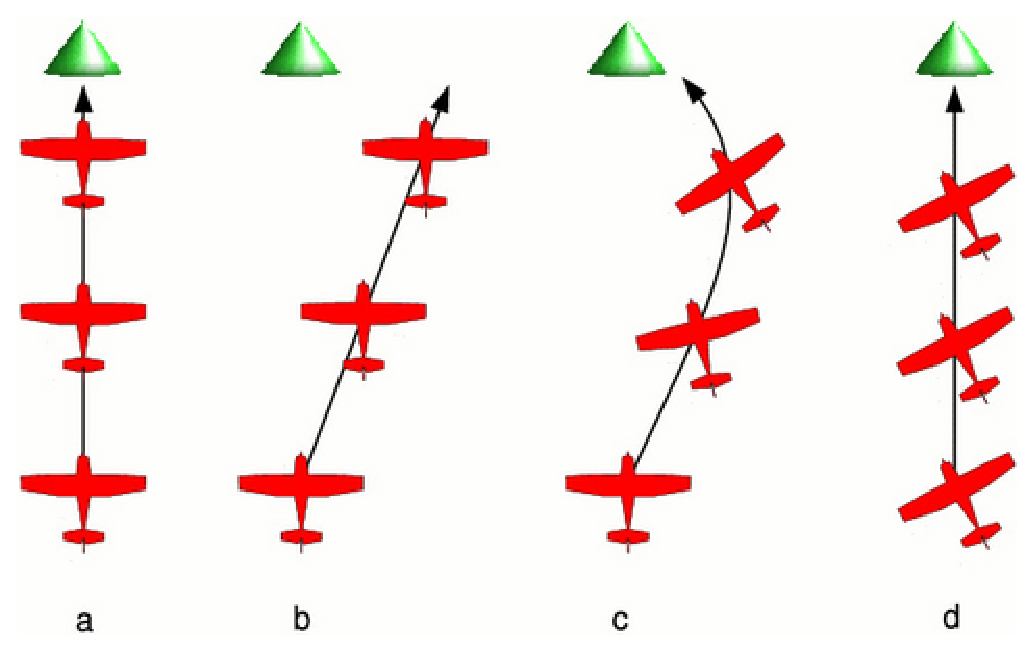
\includegraphics[width=1.0\textwidth]{img/tut_44}
\end{center}

How much to the left or to the right of the object must you head? At
what angle? Serious pilots use tight geometry and trigonometry
computations to get near exact and optimal angles. Yet I wouldn't fly a
virtual Cessna 172p if I had to do such dry things. You need no
computations at all to fly roughly straight. The trick is you must keep
your eyes on the object you fly towards. You know you will head the
plane in a direction to the left or to the right of the object, but you
don't need to know the angle. Just keep your eyes on the object. Get
aware you are drifting leftwards or rightwards. Then let your instinct
slowly head the plane to the right or to the left to compensate the
obvious drift. When you begin training this, you need to force your
instinct a little bit and think of what you are doing. Very soon this
will become automatic, just like when you learned to fly straight. You
will no more keep the plane headed towards the object. You will rather
keep it flying towards the object. The picture below shows a flight
towards the top of the little mountain ahead. Wind blows from the
right. I just look at he mountain top. And I let my hands head the
plane to right of the mountain, without really thinking about it:


\begin{center}
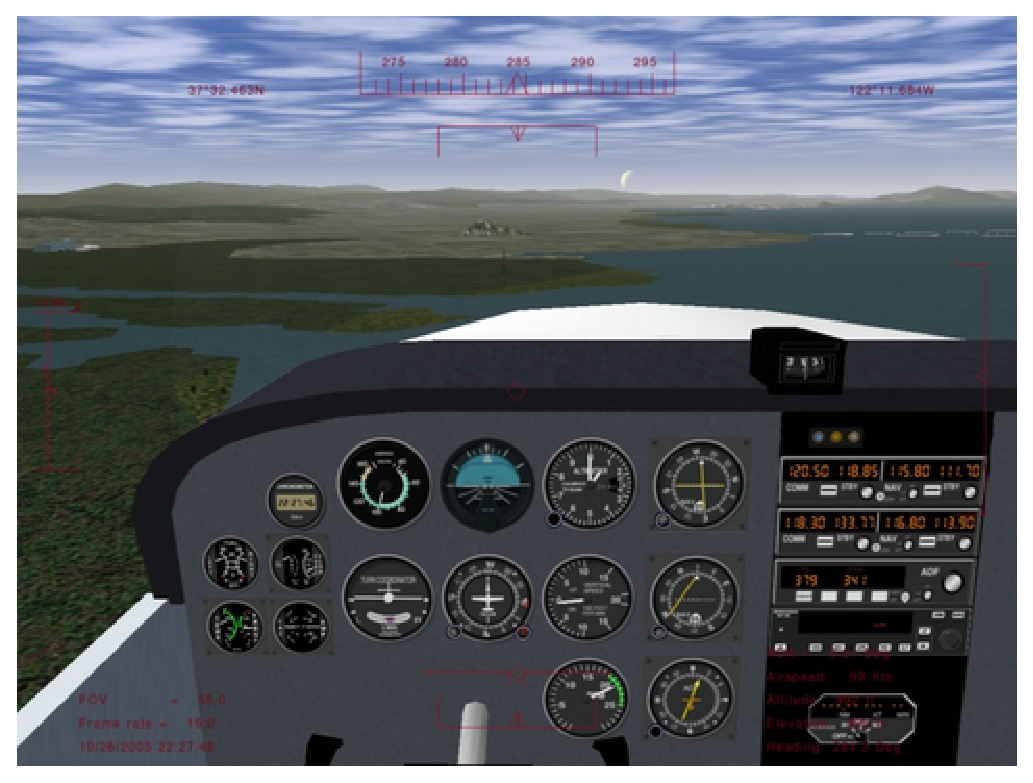
\includegraphics[width=0.5\textwidth]{img/tut_45}
\end{center}
    
    The faster the flight airspeed compared to the wind speed, the less the wind will influence.
    
    \subsection{How to take off when there is wind}
    \label{sec:Swsw}
    
Main recommendation to take off is you must find a way to accelerate
facing the wind; with the wind blowing towards the nose of the
airplane. Before most runways are build, statistics are made about the
wind at that location. The runway orientation is chosen so it aligns
with the wind most often. Lots of
\weblong{http://en.wikipedia.org/wiki/Airport}{airports} have two
runways at different orientations because the wind sometimes blows in
one of these directions and sometimes in the other direction. The
location of an airport is often chosen because at that place the wind
often has a stable direction and speed.

    
    Take off with a faint wind blowing towards the rear of the
    airplane, say 1 knot, for sure is no problem. Yet above a few knots
    you can get into trouble. With a 10 knot wind blowing from the
    rear, the front wheel will rise at the usual 40 knots airspeed, but
    that makes 50 knots compared to the runway. What matters is the
    speed the front wheel roll over the runway, not the airspeed... If
    a problem occurs and you are still rolling at 60 knots on the
    runway, the consequences will be more dramatic. To end with, you
    will need much more runway length and have less opportunities to
    abort the landing.

The main way to know the wind direction and speed is to go to the
control tower or ask the control tower by radio. A necessary and
complementary tool are the
\weblong{http://en.wikipedia.org/wiki/Windsock}{windsocks}\index{windsock}
at both ends of the runway. They show the wind direction and speed. The
longer and the stiffer the windsock, the more wind there is. The
windsock on the picture below shows an airspeed of 5 knots:
    

\begin{center}
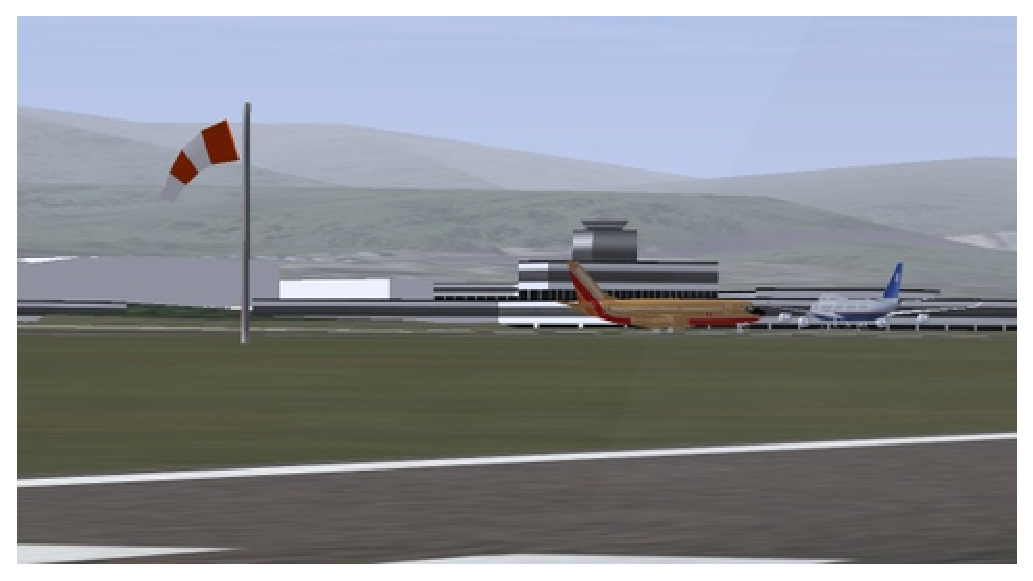
\includegraphics[width=0.5\textwidth]{img/tut_46}
\end{center}

So, you have to choose a runway start that allows you to take off with
the airplane facing the wind. In real life you are not always allowed
to do this. Either there is no runway aligned with the wind or the
control tower tells you to use another runway. Then you have to take
off under crosswind; the wind blowing towards a side of the airplane.

Basically, you can use the exact same procedure as listed above for a
take off when there is no crosswind. Yet you have to be aware of
several important facts listed below. To train this, start FlightGear
with the parameter \command{--wind=0@10} which implies a wind of 10
knots blowing from the North (direction 0). If you take off from the
usual San Francisco KSFO airport heading to the West, this makes the
wind blow from the right.


\begin{itemize}
	\item You will have to push the rudder at quite a strong angle to stay rolling aligned with the runway. Keep the rudder at that angle once the front wheel leaves the ground and a little later once the rear wheels leave the ground.

  \item Say the wind is blowing from the right. You would think you have to push the right rudder pedal, to head the airplane a little bit into the wind, to compensate for the leftwards push of the wind. Well you have to do the exact opposite: push the left rudder pedal. This is quite unnatural yet that's life. The reason of this is the rear vertical stabilizer is pushed by the wind leftwards. The plane reacts like a weather vane and heads in the wind. The plane as a whole turns to the right, with quite a strong force. You have to compensate by pushing the rudder to turn to the left. So, you take off with the ruder pedals pushed to the left. The picture below shows a rudder angle during a take off with a 10 knots crosswind blowing from the right:



\begin{center}
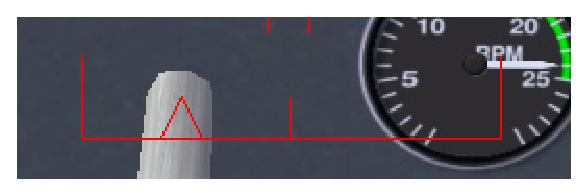
\includegraphics[width=0.5\textwidth]{img/tut_47}
\end{center}

  \item The airplane will tend to bank leftwards. Hence you will have to push the yoke/ailerons to the right. Actually you best place the yoke a little to the right before the wheels start leaving the ground. (Best is to push the yoke to the right from the start on. Indeed this is the best way to taxi safely under a crosswind blowing from the right.) The picture below shows an appropriate yoke/ailerons position, while taking off with that 10 knots crosswind blowing from the right.


\begin{center}
\includegraphics[width=0.5\textwidth]{img/tut_48}
\end{center}
  
  \item The airplane will rise in the air much slower. The vertical speed will be quite weak. This is because the rudder is at a a strong angle. The airplane moves through the air with its right flanc and brakes. You have to wait till the rudder is centered before you get the regular vertical speed. Center the rudder very slowly, a little angle step at a time. Meanwhile, using the yoke/ailerons, gradually head the airplane a little bit in the wind, to keep flying aligned with the runway. Wait till you are above a few hundreds feet before you start centering the rudder.
    
\end{itemize}   

    Why do you keep the yoke to the right and the rudder pedals to the
    left once the airplane rises in the air? This can seem odd. It's
    quite logical that way the airplane will fly straight. The ailerons
    and the rudder compensate each other and the airplane turns neither
    to the right, neither to the left. But again, why do this, why not
    simply let the yoke/ailerons and the rudder centered? The airplane
    will fly straight too and be far less braked. The reason why we do
    this is the ailerons keep the airplane banked to the right; towards
    the direction the wind is blowing from. Hence, the huge force on
    the wings, that keeps the airplane in the air, that huge force is
    now slightly directed to the right. In normal circumstances this
    would make the airplane move slowly sideways to the right, at 10
    knots speed... Currently, it compensates for the 10 knots wind and
    keeps the airplane above the runway. So despite the wind, the
    airplane stays headed towards the runway end and stays above the
    runway middle. Everything's fine (except for the braking).

To me, 10 knots wind is a maximum to take off the Cessna 172p safely.
 

    \subsection{How to land when there is wind}
    \label{sec:Lwsw}
    
    You land the Cessna 172p under crosswind the same way you take off:
      
\begin{itemize}
	\item Try to land with the wind blowing towards the airplane face. Bear in mind the wind blows the airplane away from the runway start. So start the dive later, when the engine cover already ate some length of the runway.
	\item Under crosswind, use the exact same rudder and ailerons tuning as for take off under the same crosswind. Train this by taking off and landing under crosswinds. When the wheels leave the ground and you find the appropriate yoke/ailerons angle, note down the rudder angle and the yoke/ailerons angle. Center the rudder and ailerons during the flight and make a circuit to land back. During the landing, when you fly at constant 500 feet altitude and 70 knots speed, knowing the crosswind is the same, tune in back the rudder and ailerons angle that where optimal during take off.
\end{itemize}
  
  Under high crosswind, hence with a strong rudder angle, the plane brakes a lot. This implies two things:   
    
\begin{itemize}
	\item During the approach to the runway, at constant 500 feet altitude, 70 knots speed and 1 flaps step, you need much more engine power to keep the altitude stable.
	\item Once you dive towards the runway start, keep in mind the plane is braking. So you don't need to deploy additional flaps steps. Just decrease the engine power. 
\end{itemize}
   
    Landing that way is quite comfortable, despite the crosswind. You
    just have to be a bit more careful with the rudder once the
    airplane rolls over the runway. And best keep the ailerons as if
    turning towards the wind.

Note such a landing, with a steady crosswind, is unrealistic. In the
real world the wind varies quickly. You get sudden increases and gusts
of wind. The control tower just tells you by radio the maximum speed of
the gusts. You have to adapt constantly during the landing, to react to
the turbulences and gusts.

As for the take off, 10 knots wind seems a maximum to me. (Should you
ever have to land under heavy wind, say 25 knots or more, and there is
no runway aligned with the wind, maybe best don't land on the runway.
Or don't try to align with the runway. Align exactly with the wind and
make use of the fact you need less ground length to stop. When the
plane is going to stop keep the rudder pushed. Don't try to taxi.
Simply push the parking brakes in, push the trim and get help to latch
the airplane to the ground. In fun mode, landing the Cessna 172p under
70 knots wind is great. You simply let it descent to the ground
vertically. This is quite unrealistic because at such a wind speed
there are tremendous turbulences close to the ground.)

The technique described here is the
\weblong{http://en.wikipedia.org/wiki/Slip_landing}{slip landing}.
Another crosswind landing technique is the
\weblong{http://en.wikipedia.org/wiki/Crab_landing}{crab landing}.

    
    \subsection{How to taxi when there is wind}	
    \label{sec:Twsw}	
    
    Under 10 knots wind the Cessna 172p seems not to need particular precautions when taxiing. Yet any sudden increase in wind speed can tilt it and tumble it over. So best apply the recommendations whenever there is wind. 

To train taxiing on the ground when there is wind, ask for a strong
wind like 20 knots. Such a wind can tilt the plane and blow it away
tumbling any moment. One single error during taxiing and the plane is
lost.

Main rule is you must \emph{push the yoke towards the wind}. This deserves some physical explanation: 
\begin{itemize}
	\item When the wind is blowing from 12 o'clock, this is quite logical. The yoke is pushed (towards 12 o'clock) and the elevator makes the tail rise a little. That's the most stable position to avoid the plane be tilted by the wind.
	\item When the wind comes from 10 o'clock, pushing the yoke towards 10 o'clock makes the elevator is close to centered. The elevator almost no more trades in. Now the most important part is played by the ailerons. The left aileron is upward and the right aileron is downward. This pushes the left wing down and lifts the right wing. Again, that's the most stable position to avoid the plane be tilted by the wind. 
  \item When the wind blows from 8 o'clock, you would think you should invert the position of the ailerons, to keep the left wing being pushed down. Hence you should push the yoke to 4 o'clock. Wrong! Keep pushing the yoke to 8 o'clock. The reason is the downward position of the aileron on the right wing makes it act like a \weblong{http://en.wikipedia.org/wiki/Slats}{slat}. This increases the lift on the right wing and this is all we want. Symmetrically, the upward position of the left aileron decreases the lift of the left wing.
  \item When the wind comes from the rear, from 6 o'clock, the yoke is pulled (towards 6 o'clock). The upward position of the elevator tends to make the tail be pushed down. Once again this is the best. Strong wind can push the tail against the ground. This is impressive but the tail is conceived to withstand this.
\end{itemize}
    
    Accept the plane nose can be tilted and the tail pushed against the
    ground. Keep cool. This can be impressive yet there is nothing
    dangerous with it. Go on using the brakes, rudder and engine to
    move the airplane.

If you want to move towards the wind, you will need more engine power.
When the wind blows from the rear you may need no engine power at all.
Always keep the engine power to the minimum needed.

Especially when turning, move very slowly. Make little changes at a
time. Take your time and closely survey the yoke angle. Constantly keep
it pushed towards the wind. Constantly try to reduce the engine power.
Keep in mind using the brakes too firmly may shortly tilt the plane at
an angle that allows the wind to tilt it and blow it away.
 
    \section{The autopilot}\index{autopilot}
    \label{sec:Autopilot}
    
    An \weblong{http://en.wikipedia.org/wiki/Autopilot}{autopilot} is not an ``intelligent'' pilot. It just takes over simple and wearing parts of your work as a pilot. You still are the sole real pilot aboard and have to keep aware of everything. Be prepared to shut the autopilot down. During take off and landing, relying on the autopilot would be suicidal, because you have to keep an immediate control on every function of the airplane. (Dumb autopilot systems are reported to cause less accidents than smart ones with artificial intelligence inside.)
    
    The autopilot is that little rack to the right of the yoke:
    

\begin{center}
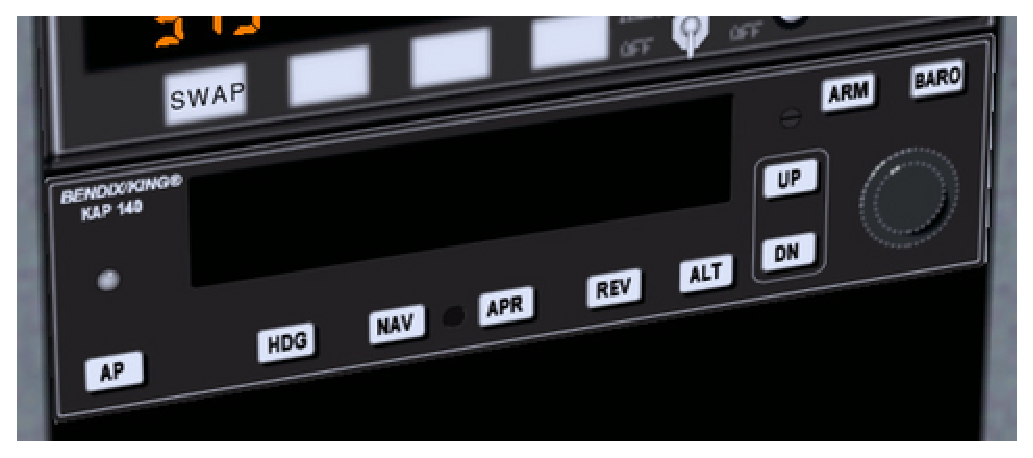
\includegraphics[width=0.5\textwidth]{img/tut_49}
\end{center}

Switch it on by pressing its  \button{AP} button (standard mouse mode).
The autopilot then controls the \index{autopilot!modes!roll control
mode}roll. It keeps the wings level with the horizon. This is displayed
in the picture below by the ``\textcolor{orange}{\button{ROL}}''marking.
To switch the autopilot down press again on \button{AP}.


\begin{center}
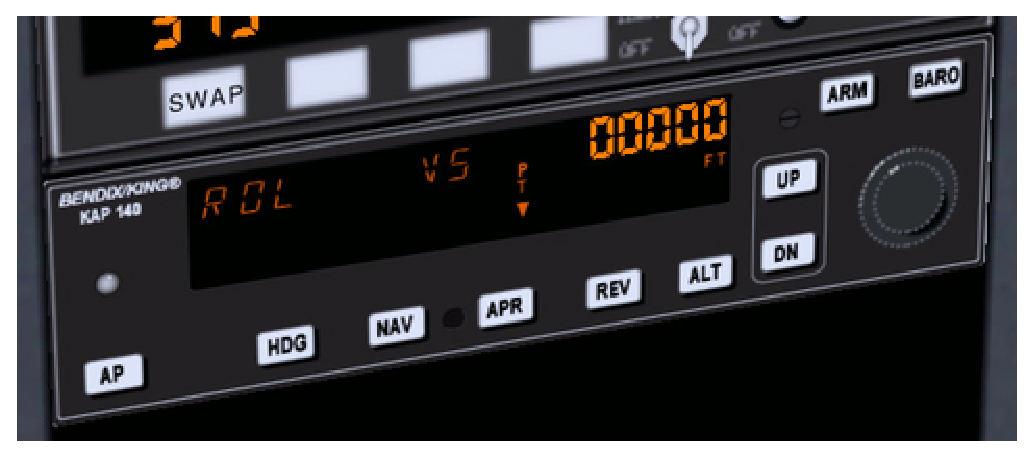
\includegraphics[width=0.5\textwidth]{img/tut_50}
\end{center}

If you press the  \button{HDG} button the autopilot will try to keep
the plane flying towards the direction tuned on the directional gyro by
the red marking (see the section \ref{sec:Kierunek} about
\index{autopilot!modes!direction mode}direction). 
``\textcolor{orange}{\button{HDG}}'' stands for ``heading''. Press
again on the \button{HDG} button to get back to roll control mode (or
\button{AP} to switch the autopilot down).


\begin{center}
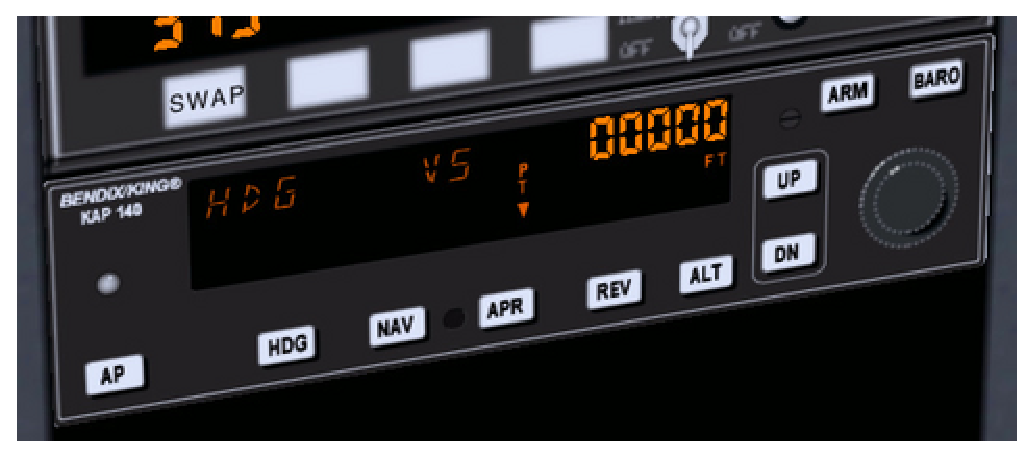
\includegraphics[width=0.5\textwidth]{img/tut_51}
\end{center}

The buttons \button{ALT}, \button{UP} and \button{DN} are used to tell
the autopilot either to control the vertical
\index{autopilot!modes!vertical speed mode}speed
\textcolor{orange}{\button{VS}} or the altitude
\textcolor{orange}{\button{ALT}}.
    
From here on you maybe better study the document used by the author of the autopilot system in FlightGear\index{autopilot!author's documentation}: 
\\[6 pt]
 \weblong{https://www3.bendixking.com/servlet/com.honeywell.aes.utility.PDFDownLoadServlet?FileName=/TechPubs/repository/006-18034-0000_2.pdf}{https://www3.bendixking.com/servlet/com.honeywell.aes.utility\\.PDFDownLoadServlet?FileName=/TechPubs/repository\\/006-18034-0000\_2.pdf}
    
    \section{Security}
    \label{sec:Bezpieczenstwo}

Security is first of all a matter of common sense. Avoid to land with
the landing gear retracted. Fill the reservoirs before take off and
don't let them get empty in flight. This may seem funny
recommendations, the fact remains I made several landings on the
aircraft belly when I started using the flight simulator. I got angry
on myself and now it nevermore happens that I forget such a simple and
essential thing. In real life you are not allowed to land airplanes on
the belly in order to get angry on yourself. I suppose it is a part of
the role of the monitors to make you feel the angriness \textbf{before}
your first solo landing. I suppose they don't let somebody fly on his
own till they feel the angriness is rooted deeply enough in him. People
who cannot cope with this are not meant to become pilots.

There are much more vital details than the landing gear and the fuel. That's why checklists exist. There are checklists for all kinds of normal or emergency situations. There a long checklists and short checklists. This link provides checklists for the Cessna 172p and for other airplanes: 
  \web{http://www.freechecklists.net/}.   Those checklists refer to much more levers, buttons and triggers than talked about in this tutorial. There is nothing complicated in those checklists provided you learned what all those little things are. For example one item is you have to verify the seats backs are upright.

  You have to learn to cope with stress. Wherever I get access to computers I try to install \fg. To me the computer industry should focus solely on building computers for \fg. Secundary tools like browsers, mailers, spreadsheets and the like, should be regarded as optional sub-functions of \fg. Once the installation is finished, I make a demo flight. Strangely, most people simply don't care about what I am doing. They just go on talking, asking questions, requesting my attention\ldots What's more I'm often not in the most adequate position toward the screen, the keyboard and the mouse. It becomes almost impossible to fly correctly, especially to land. Basically there are two possible attitudes. The first one is I get silently angry on the disturbing persons, I stop the demo and I consider it's their fault if I cannot succeed my flight. The second attitude is I breath deeply and calmly, I find ways to go on managing the burdens and the problems, I don't get angry on anybody, I claim nothing to be responsible for anything, I renounce to make a perfect demo flight and I focus on making a mediocre yet secure landing. The advantage of the first attitude is that you feel comfortable about your superiority on \fg{}-unaware persons. The disadvantage of the second attitude is that you have to endure the humiliation of an ugly landing and the people around going on talking and requesting your attention. The advantage of the second attitude is that in real life, on a real airplane, it allows you to stay alive.

Communication is a basis for security. That means communication with
the technicians, with the control tower, with your copilot, with the
passengers and especially with yourself. You have to constantly gather
data about the traffic, the meteorology and the state of mind of your
passengers. You have to constantly inform the control tower and obey
the instructions it sends you in return. You have to keep your
passengers in an acceptable mood and at the same time you have to
obtain they let you focus on your tasks when this is necessary. Lots of
airline accidents occured because of a lack of communication between
the pilot and other crew members. That has been called ``the Superman
syndrome''. Once the problems start, the pilot focuses on his way to
solve the situation. Either the copilot does not understand what the
pilot is doing or he becomes aware of a danger the pilot did not
realize. This results in contradictory commands sent to the airplane
controls, shouting, up to fist fighting\ldots till the final crash of
the airplane. An important part of the training for modern pilots is to
learn to communicate with the other crew members under high stress.
They learn to go on communicating and how to do that a short and
efficient way. (I was once told this anecdote: a monitor and a trainee
were performing landings. The trainee was a strong guy with muscles
like truck tires. At one moment the landing path appeared to be wrong.
The monitor asked the trainee to release the commands so he could take
them over. There is nothing wrong with failing a landing. Monitors
themselves sometimes fail a landing, abort and restart a new landing.
But the trainee panicked and crispated his hands on the yoke. The
monitor could do nothing. The consequence was a damaged landing gear.)

There is no room for luck in real aviation. When you train to become a
pilot, almost every possible situation is put into practice at least
once. For example a monitor makes you take off with a heavily loaded
airplane and suddenly shuts the engine down. You have to train to fly
and land with a random airplane control or indicator out of order.
\fg{} allows to reproduce some of these trainings. You can request
flight instrument failures using \fg{}s' menus or command options. A
really bad instrument failure means the instrument still seems to
operate correctly. Yet it doesn't, and what it does or displays
endangers you. While training you can decide to no more use a given
instrument or control. For example you can glue a sticker on your
screen to hide away an instrument. Best is you ask a friend to
configure a failure without you knowing what he did. This heavy
training and the numerous precautions and rules are the reason why so
few accidents occur. In most cases, even a severe problem does not lead
to an accident. Accidents are often due to the unlucky addition of
several different problems.

The picture below shows the artificial horizon indicator. I hardly
never use it. I fly looking at the real horizon. Anyway the artificial
horizon saved me more than once on the simulator. When you penetrate by
mistake in a cloud or a bank of mist, you suddenly get a white outside.
There is no more way to keep the plane flying level, except by using
the artificial horizon. You may argue this due to the lack of feedback
own to the simulator. You're (dead) wrong. The same problem occurs on a
real airplane. Quite many of the (very few) accidents in little
airplanes like the Cessna 172 or the PA-28 happen that way. It is
prohibited for a pilot with no IFR license to enter a cloud. Some do it
anyway. Or they get caught in a rise of mist the control tower didn't
warn for. The airplane banks and in two minutes time it goes flying
upside down. The pilot is unaware of this. Even worse: some instruments
seem to get mad, with no obvious reason. A crash is unavoidable. I
learned the reflex to focus on the artificial horizon, the altimeter
and the directional gyro. When this happens the plane is often already
severely banked. I keep calm and I use the instruments to maintain the
plane in a sound flight. It will oscillate a lot but serious problems
will be avoided. Either I will wait till I get out of the cloud or I
will gain or loose altitude to get out of the cloud layer. I strongly
advice you train this using the simulator. Best is you make a complete
IFR training.


\begin{center}
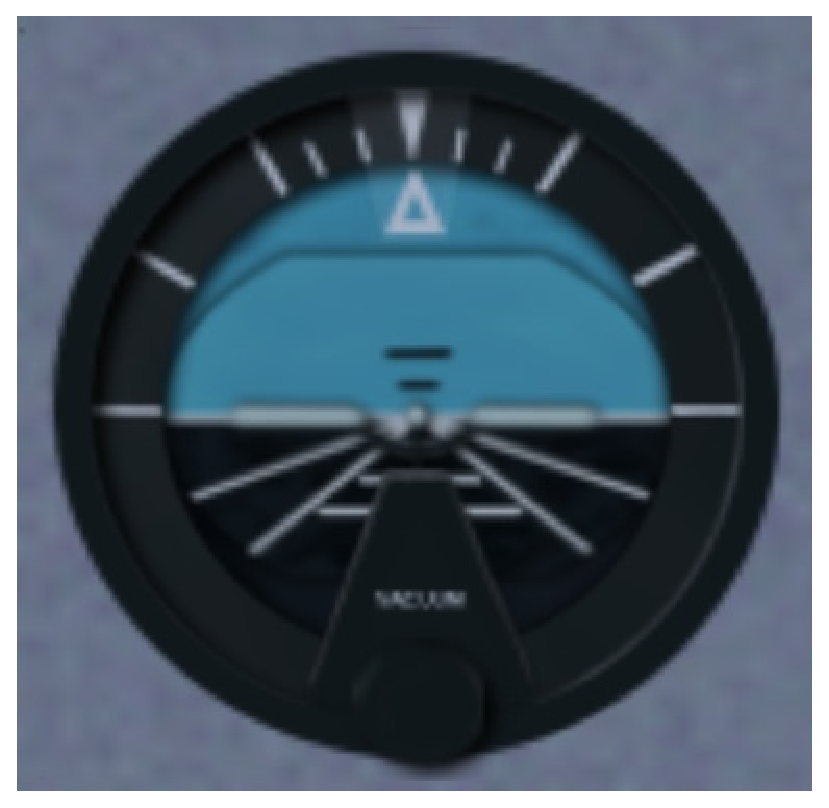
\includegraphics[width=0.25\textwidth]{img/tut_52}
\end{center}

  One thing you have to train for your security is landing on very
  short distances.\index{landing!very short distance} Some flight
  incidents, like an engine failure or a sudden change in the weather,
  can force you to land on the first strip of flat land you encounter.

The \index{HUD (Head Up Display)} HUD allows to fly and land more easily, with less stress. It also allows to optimize what you are doing and this is good for security. For example it allows to touch the ground very close after the beginning of the runway. That way you have the whole length of the runway to brake. (A HUD is available for every aircraft on FlightGear, even the 1903 Wright Flyer. In real life, few little civil airplanes contain a HUD. It is too expensive and too recent.)

There are some strong differences between a flight simulator with minimalistic control hardware and a real airplane. The fact the mouse exerts no counterforce, the fact you don't feel the vibrations and forces inside the airplane\ldots On one hand, some aspects of flying are made easier on the simulator. On the other hand, a real airplane constantly gives all sorts of valuable feedback you don't get with a simulator. One thing is common to the simulator and the real airplane: while landing you'd wish you had four arms and two more brains.

\fg{} contains bugs. Consider those problems as a training for real aircrafts. Problems on real aircrafts are not the same. But there are problems. When \fg{} suddenly puts you in a critical situation due to a bug, consider this as a training. Try to solve the situation fast and efficiently while keeping calm. It's not a bug, it's a feature!

The handbooks of airplanes contain procedures and checklists for
emergency situations. It sometime happens that the adequate reaction to
a problem is exactly the opposite for two different airplanes. That's
one reason airline pilots are not allowed to fly different airplanes at
the same time\index{aircrafts change}. If they choose to go flying
another type of airliner, there are imposed to stop flying for a
lengthy period, during which they will practice the other type of
airplane on simulators. The wide range of aircrafts available under
\fg{} allows you to experiment with this.
  
    \section{What then?}
    \label{sec:Poslowie}

Once you master the content of this tutorial, you can claim to have a
basic understanding of what piloting is about. You still lack key
knowledge and training, like these:
\begin{itemize}
	\item How to follow real checklists.
	\item How to make emergency landing on very short fields, possibly with no engine power. 
	\item How to \weblong{http://en.wikipedia.org/wiki/Navigation}{navigate} according to the rules, charts, laws, radio beacons and crosswinds.
	\item How to draw a \weblong{http://en.wikipedia.org/wiki/Flight_plan}{flight plan}.
	\item How to place the loads in an airplane to get a correct center of gravity.
	\item How to deal with the \weblong{http://en.wikipedia.org/wiki/Control_tower}{control tower} and with other airplanes.
	\item How to deal with several fuel reservoirs and their valves, pumps and backup pumps. If two reservoirs are located on the wings ends and you let one of them empty while the other keeps full, you will get severe problems. 
	\item How to deal with the failure of every possible part of the plane. 
\end{itemize}

You probably will learn to deal with a retractable
\weblong{http://en.wikipedia.org/wiki/Undercarriage}{landing gear}
system and with variable pitch
\weblong{http://en.wikipedia.org/wiki/Propeller}{propellers}.

Go to the \fg{} documentation page for more tutorials and reference
pages: \\ \web{http://www.flightgear.org/docs.html}

These are great tutorials to learn further:
\begin{itemize}
	\item \weblong{http://www.flightgear.org/Docs/Tutorials/crosscountry/tutorial.html}{http://www.flightgear.org/Docs/Tutorials/\\crosscountry/tutorial.html}
	\item \web{http://www.navfltsm.addr.com/}
\end{itemize}

I wish to thank:
\begin{itemize}
	\item Benno Schulenberg who corrected lots of mistakes in my English in this tutorial. 
	\item Albert Frank who gave me key data on piloting and corrected technical errors.
	\item Vassilii Khachaturov who learned me new things about \fg. 
	\item Roy Vegard Ovesen for pointing me to the official Autopilot Pilots Guide. 
	\item Dene Maxwell for his solution for problems under Windows Me. 
	\item Mark Akermann and Paul Surgeon for their remarks. 
	\item Michael ``Sam van der Mac'' Maciejewski who made the translation in Polish and converted the tutorial in usable \TeX{} format.
	\item The \fg{} mailing list users for their hearty welcome. 
	\item \weblong{http://www.4p8.com}{4p8} webmaster my friend Fr�d�ric Cloth for the web space used by this tutorial. 
\end{itemize}

\section{`Pilots Fly Not Only On Cessna'}
\label{sec:NieSamaCessnaPilotLata}

I cross-checked all the data about the Cessna 172p, a friend who is a
pilot verified I did not write too blatant crap and I made numerous
virtual test flights. This appendix contains less reliable data about
other airplanes. It can be helpful as an introduction to those airplanes
but keep in mind my only goal was to make flights that seem OK and
acquire basic knowledge. You need other sources if you want to pilot
these airplanes a serious way.

    \subsection{How to land the Cherokee Warrior II}
    \label{sec:Cherokee}
    
    On Linux you get the Cherokee Warrior II (or PA-28) with the   \command{--aircraft=pa28-161} command line parameter. The Cherokee Warrior II has some advantages upon the Cessna 172p. Thanks to its low wings it is far less sensitive to crosswind. Fully extended flaps are more braking and allow to land on a much shorter distance. 

Take off is the same as for the Cessna 172p (in \fg. In real life their take off checklists are not exactly the same). 

You have to get used to some minor differences of the Cherokee Warrior II for the landing:

\begin{itemize}
	\item During the steady horizontal flight before landing, the trim must be pulled a little below neutral in order to get the yoke oscillating around neutral.
	\item The optimal tachometer RPM during landing is at a lower RPM than the tachometer green zone. Roughly, keep the needle vertical.
	\item Only put one more flaps step (which makes two flaps steps deployed) when the dive towards the runway begins. Don't decrease the engine throttle too much.
	\item If you keep it to two flaps deployed during landing, the hover above the runway and the final roll will be similar to the Cessna 172p. Yet if you put the third flaps step in (after the final rounding), the plane will brake firmly. It will very quickly touch the runway then come to a near halt. Be prepared to lower the front wheel very soon. (It is possible to use the third flaps step during the dive towards the runway, instead of tuning the engine power down. Oscillating between two steps and three steps allows to aim the runway start. Yet keep two flaps steps and tune the engine seems easier. An interesting stunt is to fly stable till nearly above the runway start, then tune the engine to minimum and deploy three flaps steps. The plane almost falls to the runway. It's impressive but it works.)
\end{itemize}
    
(In real life, an advantage of the Cessna 172p upon the Cherokee
Warrior II is the fuel reservoirs of the Cessna are located in the
wings close above the center of the plane and higher than the engine.
What's more an automatic system switches between the reservoirs. That
makes you almost don't have to bother for the way the fuel gets to the
engine in flight. On the contrary, on the Cherokee Warrior II the
reservoirs are located separately, on both wings and lower than the
engine. That means you have to constantly switch between the two
reservoirs in flight. Should one reservoir become much lighter than the
other, this would destabilize the airplane. The fact the reservoirs are
lower than the engine means you have to control the fuel pumps and the
backup fuel pumps.)

Some links:\begin{itemize}
	\item \web{http://en.wikipedia.org/wiki/Piper\_Cherokee}
	\item \web{http://www.alioth.net/flying/pa28-161/index.html}
	\item \web{http://faaflyingclub.homestead.com/files/Warrior\_Checklist.pdf} 
\end{itemize}
    
    
    \subsection{How to take off and land the Piper J3 Cub}
    \label{sec:PiperJ3}
    Use the \command{--aircraft=j3cub} parameter to get the Piper J3 Cub on Linux. 

   The \weblong{http://en.wikipedia.org/wiki/Piper_J-3_Cub}{Piper J3 Cub} is a very different airplane from the Cessna 172p and the Cherokee Warrior II. The Cessna 172p and the Cherokee Warrior II are front wheel airplanes. While the Piper J3 Cub is a tail wheel airplane. Take off and landing with tail wheel airplanes is more difficult. You have to tightly use the rudder pedals when rolling over the runway. The yoke often needs to be pulled backwards to the maximum. I'll discuss this more thoroughly once I get more experience and knowledge about tail wheel airplanes. The Piper J3 Cub should be a good introduction and it is quite easy to take off and land provided you follow an appropriate procedure. Stall speed seems to be a little below 40 mph (the airspeed indicator is in mph\index{speed!units!mph [statute mile per hour]}) (about 27 knots according to the HUD). I guess an appropriate speed to rise in the air is a little above 50 mph.

My take off procedure for the Piper Cub is to fully pull the yoke
backwards then throttle the engine to maximum. Once the front wheels
clearly rises from the ground, gently push the yoke back to neutral,
towards a normal flight close above the runway. Let the plane
accelerate to 50 mph. Then pull the yoke to keep a little more than 50
mph while rising in the air.

The landing procedure\ldots well in fact there are two different landing procedures:
\begin{enumerate}
	\item The first one involves the fact the Piper J3 Cub is a very lightweight airplane. While still high in the air, throttle the engine down to minimum and slowly pull the yoke completely in while the speed decreases. This slows the plane down to stall speed (a little less than 40 mph airspeed). It makes a steep descent to the runway. Keep the yoke pulled in completely. The wings seemingly act as a parachute. The plane hits the ground and bounces on its legendary gummy landing gear. It rolls at very low speed. While still pulling the yoke in to maximum, push in the wheel brakes (key  \key{b}).
	\item Second procedure lets you land the plane like a "normal" airplane. Yet with no flaps available, at quite a lower speed and with some big differences on the yoke
\begin{itemize}
	\item Fly at say 500 feet constant altitude and "exactly" 52 mph speed towards the runway (and align with it). Let the engine cover eat up the runway start. The engine cover will hide the runway completely. To see where the runway is, push the yoke/mouse very shortly then stabilize again in normal flight.
	\item Once the runway start matches with the set of instruments (if you could see through the instrument panel), reduce the throttle to a near minimum and begin the dive towards the runway start. Keep 52 mph using the yoke. Add some throttle if you are going to miss the runway edge. (Keep in mind just a little wind is enough to change things a lot for the Piper J3 Cub).
	\item Make the rounding and pull the throttle to minimum. Do not pull steadily on the yoke. Instead let the wheels roll on the runway immediately.
	\item Once the wheels roll on the runway, \emph{push} firmly on the yoke, to its maximum. This rises the tail in the air. You would think the propeller will hit the runway or the airplane will tilt over and be damaged. But everything's fine. The wings are at a strong negative angle and this brakes the plane. (Don't push the yoke this way on other airplanes, even if their shape seems close to that of the Piper J3 Cub. Most of them will tumble forwards.)
	\item The yoke being pushed in to its maximum, push the left mouse button and keep it pushed to go in rudder control mode. Keep the plane more or less centered on the runway. This is quite uneasy. One tip is to stop aiming the rudder to say the left already when the plane just starts to turn to the left.
	\item Once the speed is really low (and the rudder control stabilized), you will see the tail begins to sink to the ground. Release the left mouse button to go back to yoke control. Pull the yoke backwards completely, to the other extreme. The tail now touches the ground and the nose is high up. Now you can use the wheel brakes (\key{b}). (If you use the brakes too early, the plane nose will hit the ground.) 
\end{itemize}
\end{enumerate}
    
    The take off procedure mentioned above is symmetrical to the first
    landing procedure. There exists a second take off procedure,
    symmetrical to the second landing procedure. Yet I don't succeed it
    properly so I won't write about it.
    
    \subsection{How to take off and land a jet}
    \label{sec:Jet}
    
    Take off on a jet is easy but you must have fast reflexes. My
    favorite jet on FlightGear is the A-4 Skyhawk. You get it with the
    \command{--aircraft=a4-uiuc} parameter on Linux, provided it is
    installed.

    This is the ``calm'' procedure to take off:
    
    
\begin{itemize}
	\item Ask for a red and full \index{HUD (Head Up Display)}\index{HUD (Head Up Display!full mode)} HUD by typing \key{h} two times. The engine throttle indicator is the leftmost on the HUD. 
	\item The airspeed indicator is the one labeled "KIAS" on the upper left side of the instrument panel. You can also use the airspeed indicator on the HUD, of course.
  \item Tune in $1\over2$ engine power.
  \item Keep the yoke pulled in $1\over2$ of its total way (picture below: the red arrow on the right side of the vertical line in the middle of the picture). 

    

\begin{center}
\includegraphics[width=0.5\textwidth]{img/tut_53}
\end{center}

  \item It is not mandatory to use the rudder to keep on the runway. The airplane will take off before it drifts off the runway. (For sure it is better and more ``secure'' to keep in the middle of the runway. But using the rudder can make things hectic for a beginner.) 
  \item Once above about 160 knots, the plane rises its nose in the air. Immediately push the yoke back to neutral or almost and stabilize at 200 knots airspeed (which makes a fair climb angle) (I've no idea whether 200 knots is the right climb speed for a real A-4. What's more I suppose one should rather use the AOA (see below).).
  \item Retract the landing gear using key  \key{g}.
  \item Either maintain $1\over2$ engine power and a speed of 200 knots to get above the clouds, or reduce the engine power to less than $1\over4$ and fly normally. (Off course you can ``fly normally'' with full engine power. Great fun.)
\end{itemize}

The ``nervous'' take off procedure is the same but you push in full
engine power. The plane takes off quickly and you need to settle a very
steep climb angle to keep 200 knots. Best retract the landing gear
immediately.

You don't land a jet the same way you land a little propeller airplane.
My way to land the A-4, inspired by some texts I found on the Web, is
this:
\begin{itemize}
	\item Really far from the runway, keep below 2,000 feet and get the speed below 200 knots. Then lower the landing gear (key \key{G}) and I deploy full flaps (all three steps, by hitting \key{]} three times).
	\item Keep a steady altitude of about 1,000 feet and a speed of ``exactly'' 150 knots. Use the mouse/yoke/elevator to tune the altitude and the engine throttle to tune the speed. (The opposite from the Cessna.)
	\item Try to align with the runway.
	\item When do you know the dive towards the runway must begin? For this you need the \index{HUD (Head Up Display)} HUD; the full default HUD with lots of features. Look at the picture below. When you see the ``distance'' between the red ``0'' lines and the runway start is 25\% the distance between the red ``0'' lines and the red ``$-10$'' dotted line, it is time to dive, aiming at the runway start. (In the picture below, that ``distance'' is 64\%, far too much to start a landing.)


\begin{center}
\includegraphics[width=0.5\textwidth]{img/tut_54}
\end{center}

Let's explain this. The two horizontal lines labeled ``0'' show the
horizon line. Rather they show where the horizon would be if the Earth
was flat. When your eyes aim at those ``0'' lines, you are looking
horizontally. Look at the dotted red lines labeled ``$-10$''. A feature
on the ground situated there is situated 10$\textdegree$ below the
ideal horizon. In other words: when you look to objects ``hidden'' by
the lines labeled ``0'', you have to lower your eyes of 10$\textdegree$
to look at objects "hidden" by the dotted lines labeled ``$-10$''. This
implies, and it is very important, that a person in a rowboat,
``hidden'' by the dotted lines labeled ``$-10$'', has to rise his eyes
up 10$\textdegree$ to look at your plane. He sees you 10$\textdegree$
above the horizon. In the picture above, the start of the runway is
situated at 64\% of the way towards the red ``-10'' dotted lines. That
means you have to lower your eyes of 6,4$\textdegree$ to look at the
runway start. This also means that if you start now to descent towards
the runway start, the descent path will be of 6,4$\textdegree$ (too
steep). So, the \index{HUD (Head Up Display)} HUD allows to measure
precisely the angle of the descent path. On a jet plane you need an
angle of 2,5$\textdegree$ (up to 3$\textdegree$), that is 25\% of
$-10\textdegree$ (up to 30\%).


\begin{center}
\includegraphics[width=0.5\textwidth]{img/tut_55}
\end{center}

	\item Once descending towards the runway start, aim at it using the yoke/mouse. And keep 150 knots speed using the engine throttle lever. 
	\item Keep measuring the angle between the ideal horizon and the runway start. It must keep 2,5$\textdegree$ (that is 25\% of  10$\textdegree$):
	  \begin{itemize}
	  \item [$\circ$] If the angle increases above 2,5$\textdegree$, you are above the desired path and you must loose altitude faster. Both decrease the engine power and dive the nose a little.
  	\item [$\circ$] If the angle decreases below  2,5$\textdegree$, you are under the desired path. I wouldn't say you should gain altitude, rather you should loose altitude less fast. Both add a little engine power and rise the nose a little. 
  \end{itemize}
	\item Once very close to the runway start, do no rounding. Don't pull steadily on the yoke like you would for the Cessna 172p. Simply let the plane touch the ground immediately, at high speed. Let it smash on the runway, so to say. All three wheels almost together. Just throttle the engine down to minimum. (If you try to pull steadily on the yoke and hover over the runway while the plane nose rises steadily, on a F-16 you would scrape the plane rear and probably destroy it.)
	\item Keep the key  \key{b} down to brake and use the rudder to stay aligned with the runway. Make only very little tunings with the rudder, otherwise the plane will tumble on one of its sides. 
\end{itemize}
    The HUD in a real jet contains a symbol to show towards what the airplane is moving. It is shown in the picture below. When you are flying at constant altitude, that symbol is on the ideal horizon line. Once you dive towards the runway start, you simply have to place that symbol on the runway start. This is quite an easy and precise way to aim at the runway start. (The diamond in the center of the FlightGear HUD sometimes can help but it does not have the same purpose. It shows towards what the airplane nose is pointing. For example is you descent towards the ground at low speed, the symbol would be somewhere on the ground while the FlightGear diamond will be up in the sky.) (By the way, the HUD on the virtual B-52 on FlightGear has that symbol. It is great to use while landing.)


\begin{center}
\includegraphics[width=0.25\textwidth]{img/tut_56}
\end{center}
Also, a real HUD shows a dotted line at  $-2,\!5\textdegree$, to help find the correct descend path. Simply keep that dotted line too on the runway start.

In a real jet you don't look at the airspeed indicator to land. Rather you look at a tool on the HUD or at the set of three lamps shown below. When the upper  $\vee$  is on, this means the speed is too slow. When the lower  $\wedge$  is on, the speed is too fast. The center  $\bigcirc$  means the speed is OK. This indicator exists in \fg. On \fg{} version 0.9.8 it seems to have wrong speeds tuned in so I didn't use it. On FlightGear version 0.9.9 it seems OK. This indicator does not rely on the speed itself. Rather it relies on the AOA. That is the Angle Of Attack, the angle at which the wings are pitched up against the relative airstream. There is a close link between the AOA and the speed. I suppose the advantage of the AOA indicator is that the optimal AOA does not depend on the plane load. While the speed does. By tuning the correct AOA, always the same for every landing, you get the optimal speed whatever the plane load. (The A-4 on \fg{} has also an AOA indicator but I don't understand its output.)


\begin{center}
\includegraphics[width=0.25\textwidth]{img/tut_57}
\end{center}

The Cessna 172 and the A-4 Skyhawk are two extremes. Most other
airplanes are in-between these two extremes. If you trained them both
(and one or two tail wheel airplanes), you should be able to find out
how to take off and land most other airplanes.

    160 knots seems an appropriate landing speed for the F-16 Falcon.
    Also you need to throttle down the engine to minimum just before
    the plane should touch the runway. Otherwise it will hover over the
    runway. Don't bother for the flaps. It seems they are deployed
    automatically with the landing gear. (Read the section
    \ref{sec:Stall} about the stall).
    
    140 up to 150 knots and all 8 flaps steps deployed seem appropriate
    to land the virtual Boeing 737. But don't trust me especially on
    that one. I just made a few experiments and didn't search for
    serious data. The landing speed varies a lot depending on the plane
    load, I suppose 140 knots is for a plane with no load. The Boeing
    737 seems to like a gentle rounding before the wheels touch the
    runway. Start the rounding early.
    
    In the take off procedure for the Cessna 172 and the A-4 Skyhawk I
    recommend you pull the yoke/mouse/elevator to $1\over2$ the total
    way, from the start on. This seems to be a bad practice on the
    Pilatus PC-7. Keep the elevator neutral. Let the plane accelerate
    and wait till the speed gets over 100 knots. Then pull calmly on
    the yoke. During landing, deploy full flaps once you start plunging
    to the runway but don't decrease the engine throttle. Decrease it
    only when the hovering above the runway starts. 100 knots seems a
    good landing speed.
    
For the Cessna 310 too you better leave the elevator neutral during the
acceleration on the runway. The plane will raise its nose by its own
provided you deployed one flaps step. (If you keep the yoke pulled from
the start on, the nose will rise sooner and you will get
\textcolor[cmyk]{0,0.25,1,0}{\textbf{y}}awful yaw problems.)
 
    (Some virtual airplanes, like some big airliners or fast aircraft,
    need faster physical computations. Then add the
    \command{--model-hz=480} parameter to the command line. If the
    plane is difficult to control during landings, try this.)

    
The angle at which you land a Cessna 172p is far steeper than the
narrow $2,5\textdegree$ for a jet. Nevertheless you are allowed to land
the Cessna at a narrow angle too. (Provided the terrain around the
runway allows for this, of course.) If you have passengers who have
ears problems with the variation of air pressure\ldots
    
    \subsection{How to take off and land the P-51D Mustang}
    \label{sec:P-51D}
    
    Should you ever get a chance to pilot a
    \weblong{http://en.wikipedia.org/wiki/P-51_Mustang}{P-51 Mustang},
    just say no. It is quite dangerous to take off and land. That's the
    kind of airplane you fly only when your country is in danger. You
    need a lot of training. Yet once in the air the P-51 Mustang seems
    no more dangerous to its pilot than other common military
    airplanes. It is quite easy to pilot.
    
    At low and medium altitude the P-51 wasn't better than the Spitfire
    and the Messerschmitts. The big difference was at high altitude.
    The P-51 kept efficient and maneuverable while enemy fighters were
    just capable to hang in the air. This was an advantage at medium
    altitude too because the P-51 was able to plunge towards enemy
    airplanes from high altitude. Another key difference was the P-51
    is very streamlined. Hence it was capable to fly much further than
    the Spitfire. These two differences let the P-51 Mustang fulfill
    its purpose: escort Allied bombers all the way to their targets in
    Germany. This allowed the bombings to be much more efficient and
    contributed to the defeat of the Nazis.
    
    To get the The P-51D Mustang in Linux use the
    \command{--aircraft=p51d} command line parameter.
    
    To take off the P-51D Mustang in \fg, deploy one flaps step, pull
    and keep the yoke completely backwards, push the engine throttle to
    maximum and keep the left mouse button pressed to control the
    rudder and keep on the runway. Once you reach exactly 100 mph,
    suddenly push the rudder 1/3 of its total way to the right.
    Immediately release the left mouse button and push the yoke to rise
    the tail (don't push it too much, as the sooner the wheels leave
    the ground the better). From now on, keep the left mouse button
    released. Only make very short adjustments to the rudder. Let the
    plane rise from the runway and get to altitude at a speed of say
    150 mph. Don't forget to retract the landing gear and the flaps.

Don't make too steep turns. You would loose control on the plane and crash.

To land, deploy full flaps and lower the landing gear from the start
on. 130 mph speed seems fine, up to 140 mph. Make an approach from
1,000 feet altitude and a dive at a low angle, like for a jet. Once
over the runway, shut the engine down completely (key{\{}). Don't hover
over the runway. Get the wheels rolling soon (like for a jet). Hold the
left mouse button down to steer the plane using the rudder. Once the
tail sinks in, briskly pull the yoke (left mouse button shortly
released) to force the tail on the runway. Go on steering the plane
using the rudder. Now the tail is firmly on the ground, use the brakes
if you want.
    
    \subsection{How to take off and land the B-52 Stratofortress}
    \label{sec:B52}
  
  The B-52F bomber implemented in \fg is a success. It is one of my
  favorite airplanes. I'm sorry it was conceived to terrify me. One
  single B-52 bomber can wipe out every main town of my country and
  rise a nightmare of sicknesses and children malformation for
  centuries. All B-52 bombers united can wipe out mankind and almost
  every kinds of plants and animals on Earth.
  
  The differences between the virtual B-52F bomber and the Cessna 172p are these:
\begin{itemize}
	\item The B-52F starts with the flaps deployed and the parking brakes set.
	\item There are only two flaps steps: retracted and deployed. When deployed they are only meant to make the wings lift more, not to brake. If you want to brake, you need the spoilers. They deploy on the the upper side of the wings. Use the key \key{k} to deploy the spoilers and the key \key{j} to retract them. There are seven steps of spoilers.
	\item The main landing gear of the Cessna 172p is composed of two wheels, one on each side of the airplane. In order for these wheels to leave and touch the ground altogether, you need to keep the wings parallel with the ground. The main landing gear of the B-52F is composed of a set of wheels at the front and a set of wheels at the rear. This implies that in order for these wheels to leave and touch the ground altogether, you need to keep the airplane body parallel with the ground. 
\end{itemize}
This is my procedure to take off the virtual B-52F:
\begin{itemize}
	\item \emph{Push} the yoke  $1\over3$ of the total way.
	\item Push the engine throttle to maximum.
	\item Release the parking brakes (key \key{B}).
	\item Push down the left mouse button to control the rudder pedals and keep the airplane on the runway
	\item The whole runway length is needed till the B-52F rises from the ground (KSFO).
	\item Once the B-52F leaves the ground, around 190 knots seems appropriate to get to altitude.
	\item Retract the flaps and the landing gear. 
\end{itemize}

To land, the B-52F's HUD offers that great airplane-shaped symbol I
talked about in the section about jets. So you just have to put that
symbol on the airplane threshold (a few pixels further seems optimal)
and keep the runway start 2,5$\textdegree$ below the ideal horizon
line. 130 up to 140 knots seems a good landing speed. (Instead of the
speed you can make use of the AOA indicator displayed on the schematic
instrument panel (\key{P}). ). Simply keep the AOA at 3$\textdegree$. I
must confess I prefer to tune the speed rather than the AOA.) If the
plane gets to the runway at 130 up to 140 knots, simply ``let it
smash'' on the runway. Otherwise, if the speed is higher, make a
rounding and a short hover. The brakes seem to be very effective
\key{b}). They allow to stop the B-52F on roughly the same short runway
length as the Cessna 172p.

Replays of the flights are a delight. They allow to check the plane
body left the runway and landed back parallel with it. One of the
points of view is situated inside the B-52F rear turret, which allows
you to be your own passenger and to compare what you see with what you
experienced as a passenger in airliners. The key \key{K} allows to
visualize the airplane trajectory.

To cause an accident with the B-52 do this:
\begin{itemize}
	\item Make a steep turn with a very strong bank; the wings nearly perpendicular to the ground.
	\item Try to get the plane back level. It will obey but very slowly. You will get aware that the turn will go on for a while and that you will turn further than your intended flight direction.
	\item Do something that accelerates the stabilization on some airplanes: push the rudder to an extreme, opposite to the current turn. This will suddenly make the airplane drop from the sky. 
\end{itemize}
